\documentclass{article}
\usepackage{amsmath, amssymb, graphicx, geometry, tikz, array, booktabs, enumitem, listings, xcolor, fancyhdr, float, subcaption, hyperref}

\title{Module 6: The Perceptron Algorithm}
\author{Machine Learning Course}
\date{}

\begin{document}

\maketitle
\tableofcontents
\newpage

\section{Introduction to the Perceptron}

\subsection{Historical Context}
The Perceptron algorithm is one of the earliest and most influential algorithms in machine learning. It was developed in the late 1950s by Frank Rosenblatt, inspired by the functioning of a biological neuron. Despite its simplicity, the Perceptron laid the groundwork for many modern machine learning techniques, including neural networks and deep learning.

\subsection{From Linear Boundaries to Learning Algorithms}
In previous discussions, we explored linear boundaries for binary classification:
\begin{itemize}
    \item Data points $\mathbf{x} \in \mathbb{R}^d$ with binary labels $y \in \{-1, +1\}$
    \item Linear decision boundaries defined by $\mathbf{w} \cdot \mathbf{x} + b = 0$
    \item Prediction rule: $\hat{y} = \text{sign}(\mathbf{w} \cdot \mathbf{x} + b)$
\end{itemize}

The Perceptron algorithm provides a systematic way to learn the parameters $\mathbf{w}$ and $b$ from training data.

\section{Linear Classification Revisited}

\subsection{Binary Classification Framework}
\begin{itemize}
    \item Input: Feature vectors $\mathbf{x} \in \mathbb{R}^d$
    \item Output: Binary labels $y \in \{-1, +1\}$
    \item Goal: Learn a linear decision boundary that separates positive from negative examples
\end{itemize}

\subsection{Linear Classifier Parameters}
A linear classifier is defined by:
\begin{itemize}
    \item Weight vector $\mathbf{w} \in \mathbb{R}^d$
    \item Bias term $b \in \mathbb{R}$
\end{itemize}

\subsection{Prediction and Correctness}
For a data point $\mathbf{x}$ with true label $y$:
\begin{itemize}
    \item Prediction: $\hat{y} = \text{sign}(\mathbf{w} \cdot \mathbf{x} + b)$
    \item Classifier is correct if $y = \hat{y}$
    \item Equivalently, classifier is correct if $y(\mathbf{w} \cdot \mathbf{x} + b) > 0$
\end{itemize}

This last formulation is particularly useful for the Perceptron algorithm.

\section{Loss Function for Classification}

\subsection{Defining the Loss}
To learn a linear classifier, we need to define a loss function that quantifies how "wrong" our model is on a given example.

For a point $(\mathbf{x}, y)$, a natural loss function is:
\begin{itemize}
    \item If $y(\mathbf{w} \cdot \mathbf{x} + b) > 0$ (correct prediction): Loss = 0
    \item If $y(\mathbf{w} \cdot \mathbf{x} + b) \leq 0$ (incorrect prediction): Loss = $-y(\mathbf{w} \cdot \mathbf{x} + b)$
\end{itemize}

This loss function has several desirable properties:
\begin{itemize}
    \item Zero loss for correct predictions
    \item Positive loss for incorrect predictions
    \item Higher loss for predictions that are "more wrong"
\end{itemize}

\subsection{Example of Loss Calculation}
\begin{itemize}
    \item Suppose $y = -1$ (true label) and $\mathbf{w} \cdot \mathbf{x} + b = 0.1$
    \item We predict $\hat{y} = +1$ (incorrect)
    \item Loss = $-(-1)(0.1) = 0.1$ (small loss)
\end{itemize}

\begin{itemize}
    \item Suppose $y = -1$ (true label) and $\mathbf{w} \cdot \mathbf{x} + b = 10$
    \item We predict $\hat{y} = +1$ (incorrect)
    \item Loss = $-(-1)(10) = 10$ (large loss)
\end{itemize}

\section{Stochastic Gradient Descent}

\subsection{Optimization Approach}
To find the optimal parameters $\mathbf{w}$ and $b$, we use stochastic gradient descent (SGD):
\begin{itemize}
    \item Process one training example at a time
    \item Update parameters in the direction that reduces the loss
    \item Repeat until convergence
\end{itemize}

\subsection{Gradient of the Loss}
For the loss function defined above:
\begin{itemize}
    \item If $y(\mathbf{w} \cdot \mathbf{x} + b) > 0$ (correct): Gradient = 0 (no update)
    \item If $y(\mathbf{w} \cdot \mathbf{x} + b) \leq 0$ (incorrect):
    \begin{itemize}
        \item Gradient with respect to $\mathbf{w}$ is $-y\mathbf{x}$
        \item Gradient with respect to $b$ is $-y$
    \end{itemize}
\end{itemize}

\subsection{Update Rules}
The SGD update rules are:
\begin{itemize}
    \item $\mathbf{w} = \mathbf{w} + \alpha y\mathbf{x}$
    \item $b = b + \alpha y$
\end{itemize}
where $\alpha$ is the learning rate (step size).

For simplicity, the Perceptron algorithm uses $\alpha = 1$.

\section{The Perceptron Algorithm}

\subsection{Algorithm Description}
\fbox{
\begin{minipage}{\dimexpr\textwidth-2\fboxsep-2\fboxrule\relax}
\textbf{The Perceptron Algorithm}
\begin{enumerate}
    \item Initialize $\mathbf{w} = \mathbf{0}$ and $b = 0$
    \item Repeat until convergence:
    \begin{enumerate}
        \item For each training example $(\mathbf{x}, y)$:
        \begin{enumerate}
            \item If $y(\mathbf{w} \cdot \mathbf{x} + b) \leq 0$ (misclassified):
            \begin{enumerate}
                \item $\mathbf{w} = \mathbf{w} + y\mathbf{x}$
                \item $b = b + y$
            \end{enumerate}
        \end{enumerate}
    \end{enumerate}
\end{enumerate}
\end{minipage}
}

\subsection{Intuitive Explanation}
The Perceptron algorithm has an intuitive interpretation:
\begin{itemize}
    \item If a positive example ($y = +1$) is misclassified, add its feature vector to $\mathbf{w}$ and increase $b$
    \item If a negative example ($y = -1$) is misclassified, subtract its feature vector from $\mathbf{w}$ and decrease $b$
\end{itemize}

This gradually adjusts the decision boundary to correctly classify more training examples.

\begin{figure}[h]
\centering
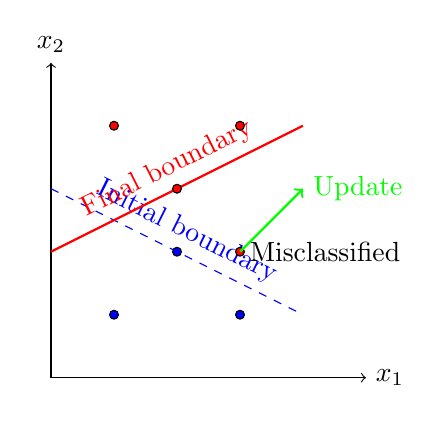
\begin{tikzpicture}[scale=0.8]
    \draw[->] (0,0) -- (5,0) node[right] {$x_1$};
    \draw[->] (0,0) -- (0,5) node[above] {$x_2$};
    
    % Initial boundary
    \draw[dashed, blue] (0,3) -- (4,1) node[midway, above, sloped] {Initial boundary};
    
    % Final boundary
    \draw[thick, red] (0,2) -- (4,4) node[midway, above, sloped] {Final boundary};
    
    % Points
    \draw[fill=red] (1,4) circle (2pt);
    \draw[fill=red] (2,3) circle (2pt);
    \draw[fill=red] (3,4) circle (2pt);
    \draw[fill=blue] (1,1) circle (2pt);
    \draw[fill=blue] (2,2) circle (2pt);
    \draw[fill=blue] (3,1) circle (2pt);
    
    % Misclassified point
    \draw[fill=red] (3,2) circle (2pt) node[right] {Misclassified};
    \draw[->, thick, green] (3,2) -- (4,3) node[right] {Update};
\end{tikzpicture}
\caption{Illustration of a Perceptron update. The misclassified positive point causes the decision boundary to shift.}
\end{figure}

\section{The Perceptron in Action}

\subsection{Example: Linearly Separable Data}
The lecture demonstrated the Perceptron algorithm on a dataset of 85 linearly separable points:
\begin{itemize}
    \item The algorithm was run multiple times with different random orderings of the data
    \item Each run converged to a different linear boundary that perfectly separated the classes
    \item The number of iterations required for convergence varied (e.g., 9, 15, 8, 14 iterations)
\end{itemize}

\subsection{Visualization of Convergence}
\begin{figure}[h]
\centering
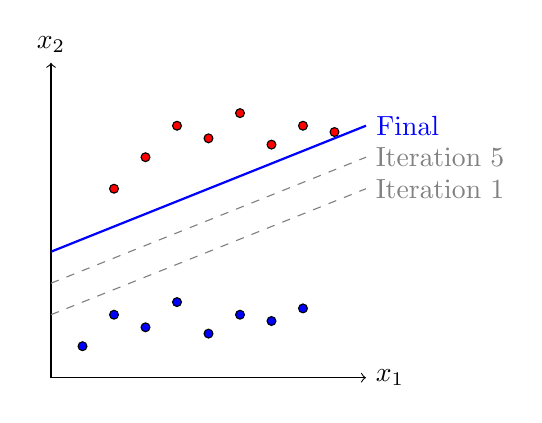
\begin{tikzpicture}[scale=0.8]
    % Coordinate axes
    \draw[->] (0,0) -- (5,0) node[right] {$x_1$};
    \draw[->] (0,0) -- (0,5) node[above] {$x_2$};
    
    % Data points (simplified representation)
    \foreach \x/\y in {0.5/0.5, 1/1, 1.5/0.8, 2/1.2, 2.5/0.7, 3/1, 3.5/0.9, 4/1.1}
        \draw[fill=blue] (\x,\y) circle (2pt);
    
    \foreach \x/\y in {1/3, 1.5/3.5, 2/4, 2.5/3.8, 3/4.2, 3.5/3.7, 4/4, 4.5/3.9}
        \draw[fill=red] (\x,\y) circle (2pt);
    
    % Decision boundaries at different iterations
    \draw[dashed, gray] (0,1) -- (5,3) node[right] {Iteration 1};
    \draw[dashed, gray] (0,1.5) -- (5,3.5) node[right] {Iteration 5};
    \draw[thick, blue] (0,2) -- (5,4) node[right] {Final};
\end{tikzpicture}
\caption{Illustration of Perceptron convergence on linearly separable data. The decision boundary evolves over iterations until it perfectly separates the classes.}
\end{figure}

\section{Convergence Properties}

\subsection{Convergence Theorem}
A fundamental result for the Perceptron algorithm:

\fbox{
\begin{minipage}{\dimexpr\textwidth-2\fboxsep-2\fboxrule\relax}
\textbf{Perceptron Convergence Theorem}

If the training data is linearly separable, then:
\begin{itemize}
    \item The Perceptron algorithm will find a linear classifier with zero training error
    \item It will converge within a finite number of steps
\end{itemize}
\end{minipage}
}

\subsection{Margin and Convergence Rate}
The number of iterations required for convergence depends on the margin:
\begin{itemize}
    \item Margin: A measure of the separation between the two classes
    \item Larger margin → Faster convergence
    \item The upper bound on the number of iterations is proportional to $1/\gamma^2$, where $\gamma$ is the margin
\end{itemize}

\begin{figure}[h]
\centering
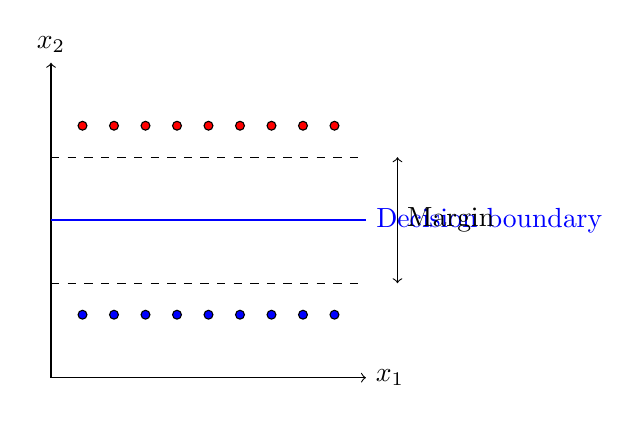
\begin{tikzpicture}[scale=0.8]
    \draw[->] (0,0) -- (5,0) node[right] {$x_1$};
    \draw[->] (0,0) -- (0,5) node[above] {$x_2$};
    
    % Decision boundary
    \draw[thick, blue] (0,2.5) -- (5,2.5) node[right] {Decision boundary};
    
    % Margin
    \draw[dashed] (0,1.5) -- (5,1.5);
    \draw[dashed] (0,3.5) -- (5,3.5);
    \draw[<->] (5.5,1.5) -- (5.5,3.5) node[midway, right] {Margin};
    
    % Points
    \foreach \x in {0.5,1,...,4.5}
        \draw[fill=blue] (\x,1) circle (2pt);
    
    \foreach \x in {0.5,1,...,4.5}
        \draw[fill=red] (\x,4) circle (2pt);
\end{tikzpicture}
\caption{Illustration of margin in a linearly separable dataset. The margin is the distance between the decision boundary and the closest data points.}
\end{figure}

\section{Limitations and Extensions}

\subsection{Non-linearly Separable Data}
The Perceptron algorithm has a significant limitation:
\begin{itemize}
    \item It is only guaranteed to converge if the data is linearly separable
    \item For non-linearly separable data, it may oscillate indefinitely
\end{itemize}

\subsection{Pocket Algorithm}
A simple extension to handle non-linearly separable data:
\begin{itemize}
    \item Run the standard Perceptron algorithm
    \item Keep track of the best weights found so far (those with the lowest training error)
    \item Return these "pocket" weights after a fixed number of iterations
\end{itemize}

\subsection{Kernel Perceptron}
The Perceptron can be extended to handle non-linear decision boundaries using the kernel trick:
\begin{itemize}
    \item Implicitly map the data to a higher-dimensional space where it becomes linearly separable
    \item Apply the Perceptron algorithm in this higher-dimensional space
    \item Common kernels: polynomial, radial basis function (RBF)
\end{itemize}

\begin{figure}[h]
\centering
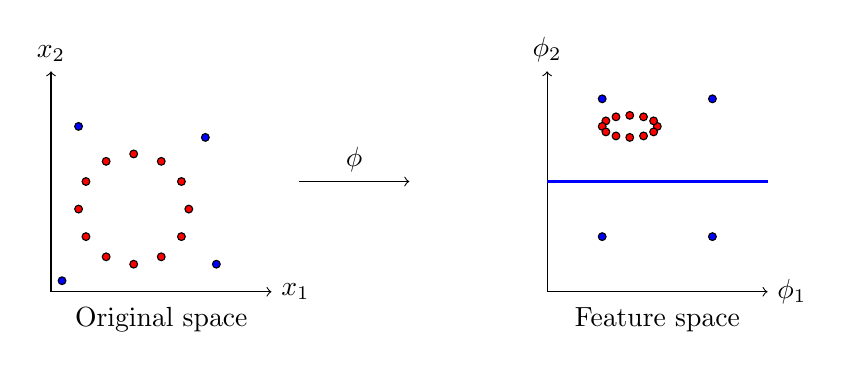
\begin{tikzpicture}[scale=0.7]
    % Original space
    \begin{scope}
        \draw[->] (0,0) -- (4,0) node[right] {$x_1$};
        \draw[->] (0,0) -- (0,4) node[above] {$x_2$};
        
        % Circle of points
        \foreach \angle in {0,30,...,330}
            \draw[fill=red] ({1.5+cos(\angle)},{1.5+sin(\angle)}) circle (2pt);
        
        % Outer points
        \foreach \x/\y in {0.2/0.2, 0.5/3, 3/0.5, 2.8/2.8}
            \draw[fill=blue] (\x,\y) circle (2pt);
        
        \node at (2,-0.5) {Original space};
    \end{scope}
    
    % Arrow
    \draw[->] (4.5,2) -- (6.5,2) node[midway, above] {$\phi$};
    
    % Feature space
    \begin{scope}[xshift=9cm]
        \draw[->] (0,0) -- (4,0) node[right] {$\phi_1$};
        \draw[->] (0,0) -- (0,4) node[above] {$\phi_2$};
        
        % Transformed points
        \foreach \angle in {0,30,...,330}
            \draw[fill=red] ({1.5+0.5*cos(\angle)},{3+0.2*sin(\angle)}) circle (2pt);
        
        \foreach \x/\y in {1/1, 1/3.5, 3/1, 3/3.5}
            \draw[fill=blue] (\x,\y) circle (2pt);
        
        % Linear separator
        \draw[thick, blue] (0,2) -- (4,2);
        
        \node at (2,-0.5) {Feature space};
    \end{scope}
\end{tikzpicture}
\caption{Kernel trick: Mapping non-linearly separable data to a space where it becomes linearly separable}
\end{figure}

\section{Relationship to Neural Networks}

\subsection{The Perceptron as a Neuron}
The Perceptron can be viewed as a single artificial neuron:
\begin{itemize}
    \item Inputs: Feature vector $\mathbf{x}$
    \item Weights: Vector $\mathbf{w}$ and bias $b$
    \item Activation function: Sign function
    \item Output: Binary prediction $\hat{y}$
\end{itemize}

\subsection{Multi-layer Perceptrons}
Modern neural networks extend the Perceptron concept:
\begin{itemize}
    \item Multiple layers of neurons
    \item Differentiable activation functions (e.g., sigmoid, ReLU)
    \item Trained using backpropagation and gradient descent
\end{itemize}

\begin{figure}[h]
\centering
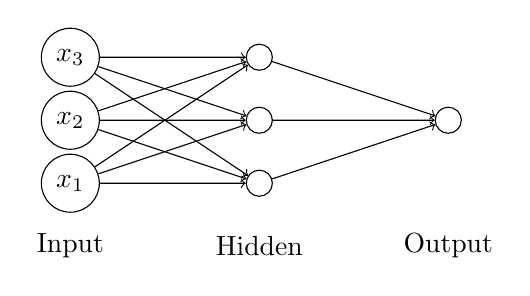
\begin{tikzpicture}[scale=0.8]
    % Input layer
    \foreach \i in {1,2,3} {
        \node[circle, draw] (I\i) at (0,\i) {$x_\i$};
    }
    \node at (0,0) {Input};
    
    % Hidden layer
    \foreach \i in {1,2,3} {
        \node[circle, draw] (H\i) at (3,\i) {};
    }
    \node at (3,0) {Hidden};
    
    % Output layer
    \node[circle, draw] (O1) at (6,2) {};
    \node at (6,0) {Output};
    
    % Connections
    \foreach \i in {1,2,3} {
        \foreach \j in {1,2,3} {
            \draw[->] (I\i) -- (H\j);
        }
    }
    
    \foreach \i in {1,2,3} {
        \draw[->] (H\i) -- (O1);
    }
\end{tikzpicture}
\caption{A multi-layer perceptron with one hidden layer}
\end{figure}

\section{Worked Examples}

\subsection{Example 1: Perceptron Learning on a Simple Dataset}
Consider the following 2D dataset:
\begin{itemize}
    \item Positive examples: $(1,1)$, $(2,2)$
    \item Negative examples: $(1,2)$, $(2,1)$
\end{itemize}

Let's trace through the Perceptron algorithm:

\paragraph{Initialization:} $\mathbf{w} = (0,0)$, $b = 0$

\paragraph{Iteration 1:}
\begin{itemize}
    \item Example $(1,1)$, $y = +1$:
    \begin{align}
        y(\mathbf{w} \cdot \mathbf{x} + b) &= 1 \cdot ((0,0) \cdot (1,1) + 0) = 0 \leq 0
    \end{align}
    Misclassified, so update:
    \begin{align}
        \mathbf{w} &= (0,0) + 1 \cdot (1,1) = (1,1)\\
        b &= 0 + 1 = 1
    \end{align}
    
    \item Example $(2,2)$, $y = +1$:
    \begin{align}
        y(\mathbf{w} \cdot \mathbf{x} + b) &= 1 \cdot ((1,1) \cdot (2,2) + 1) = 5 > 0
    \end{align}
    Correctly classified, no update.
    
    \item Example $(1,2)$, $y = -1$:
    \begin{align}
        y(\mathbf{w} \cdot \mathbf{x} + b) &= -1 \cdot ((1,1) \cdot (1,2) + 1) = -4 < 0
    \end{align}
    Correctly classified, no update.
    
    \item Example $(2,1)$, $y = -1$:
    \begin{align}
        y(\mathbf{w} \cdot \mathbf{x} + b) &= -1 \cdot ((1,1) \cdot (2,1) + 1) = -4 < 0
    \end{align}
    Correctly classified, no update.
\end{itemize}

After one pass through the data, all examples are correctly classified. The final decision boundary is $x_1 + x_2 + 1 = 0$ or $x_2 = -x_1 - 1$.

\subsection{Example 2: Non-convergence on Non-linearly Separable Data}
Consider the XOR problem:
\begin{itemize}
    \item Positive examples: $(0,0)$, $(1,1)$
    \item Negative examples: $(0,1)$, $(1,0)$
\end{itemize}

This dataset is not linearly separable. Let's see what happens with the Perceptron:

\paragraph{Initialization:} $\mathbf{w} = (0,0)$, $b = 0$

\paragraph{Iteration 1:}
\begin{itemize}
    \item Example $(0,0)$, $y = +1$:
    \begin{align}
        y(\mathbf{w} \cdot \mathbf{x} + b) &= 1 \cdot ((0,0) \cdot (0,0) + 0) = 0 \leq 0
    \end{align}
    Misclassified, so update:
    \begin{align}
        \mathbf{w} &= (0,0) + 1 \cdot (0,0) = (0,0)\\
        b &= 0 + 1 = 1
    \end{align}
    
    \item Example $(1,1)$, $y = +1$:
    \begin{align}
        y(\mathbf{w} \cdot \mathbf{x} + b) &= 1 \cdot ((0,0) \cdot (1,1) + 1) = 1 > 0
    \end{align}
    Correctly classified, no update.
    
    \item Example $(0,1)$, $y = -1$:
    \begin{align}
        y(\mathbf{w} \cdot \mathbf{x} + b) &= -1 \cdot ((0,0) \cdot (0,1) + 1) = -1 < 0
    \end{align}
    Correctly classified, no update.
    
    \item Example $(1,0)$, $y = -1$:
    \begin{align}
        y(\mathbf{w} \cdot \mathbf{x} + b) &= -1 \cdot ((0,0) \cdot (1,0) + 1) = -1 < 0
    \end{align}
    Correctly classified, no update.
\end{itemize}

At this point, $\mathbf{w} = (0,0)$ and $b = 1$, which classifies everything as positive. This is clearly not correct for the negative examples. If we continue iterating, the algorithm will keep updating without converging to a solution that correctly classifies all examples.

\section{Practical Considerations}

\subsection{Initialization}
While the standard Perceptron initializes $\mathbf{w} = \mathbf{0}$ and $b = 0$, different initializations can lead to different solutions and convergence rates.

\subsection{Data Ordering}
The order in which training examples are processed can significantly impact:
\begin{itemize}
    \item The number of iterations required for convergence
    \item The specific decision boundary found
\end{itemize}
Randomizing the order of examples between epochs is a common practice.

\subsection{Learning Rate}
While the standard Perceptron uses a learning rate of 1, a smaller learning rate can sometimes lead to more stable convergence, especially in noisy settings.

\subsection{Feature Scaling}
As with most linear models, the Perceptron benefits from feature scaling:
\begin{itemize}
    \item Standardization: $x' = \frac{x - \mu}{\sigma}$
    \item Min-max scaling: $x' = \frac{x - \min(x)}{\max(x) - \min(x)}$
\end{itemize}

\section{Summary and Key Takeaways}

\subsection{Core Concepts}
\begin{itemize}
    \item The Perceptron is an algorithm for learning linear classifiers
    \item It updates the model parameters only when a misclassification occurs
    \item The update rule is simple: add the feature vector (scaled by the label) to the weight vector
    \item For linearly separable data, the Perceptron is guaranteed to converge in a finite number of steps
\end{itemize}

\subsection{Strengths}
\begin{itemize}
    \item Simple and intuitive algorithm
    \item Guaranteed convergence for linearly separable data
    \item Online learning capability (can process one example at a time)
    \item Historically significant as a foundation for neural networks
\end{itemize}

\subsection{Limitations}
\begin{itemize}
    \item Only works for linearly separable data
    \item No convergence guarantee for non-linearly separable data
    \item The solution depends on the order of training examples
    \item Does not provide probability estimates
\end{itemize}

\subsection{Extensions and Related Concepts}
\begin{itemize}
    \item Pocket Algorithm for non-linearly separable data
    \item Kernel Perceptron for non-linear decision boundaries
    \item Multi-layer Perceptrons and neural networks
    \item Support Vector Machines for maximum-margin linear classification
\end{itemize}

\end{document}\documentclass{article}
\usepackage{amsmath, amssymb, graphicx, geometry, tikz, array, booktabs, enumitem, listings, xcolor, fancyhdr, float, subcaption, hyperref}

\title{Module 6: Maximizing the Margin of a Linear Classifier\\(Support Vector Machines)}
\author{Machine Learning Course}
\date{}

\begin{document}

\maketitle
\tableofcontents
\newpage

\section{Introduction to Support Vector Machines}

\subsection{From Perceptron to Maximum-Margin Classifiers}
In the previous lecture, we explored the Perceptron algorithm, which finds a linear decision boundary that correctly classifies all training examples (assuming the data is linearly separable). However, the Perceptron algorithm has a key limitation: it can find any linear separator that works, but it doesn't necessarily find the "best" one.

This raises an important question: Among all possible linear separators, which one should we choose? Support Vector Machines (SVMs) provide a principled answer to this question by finding the linear separator that maximizes the margin between the two classes.

\subsection{Motivation for Maximum-Margin Classification}
Why should we care about maximizing the margin? There are several compelling reasons:

\begin{itemize}
    \item \textbf{Generalization}: A classifier with a larger margin is likely to generalize better to unseen data
    \item \textbf{Robustness}: Maximum-margin classifiers are more robust to small perturbations in the data
    \item \textbf{Theoretical guarantees}: The margin is directly related to bounds on the generalization error
    \item \textbf{Uniqueness}: Unlike the Perceptron, which can find many different solutions, the maximum-margin classifier is unique (for linearly separable data)
\end{itemize}

\section{Review of Linear Classification}

\subsection{The Perceptron Algorithm}
Let's briefly review the Perceptron algorithm:

\fbox{
\begin{minipage}{\dimexpr\textwidth-2\fboxsep-2\fboxrule\relax}
\textbf{The Perceptron Algorithm}
\begin{enumerate}
    \item Initialize $\mathbf{w} = \mathbf{0}$ and $b = 0$
    \item Keep cycling through the training data $(\mathbf{x}, y)$:
    \begin{enumerate}
        \item If $y(\mathbf{w} \cdot \mathbf{x} + b) \leq 0$ (i.e., point misclassified):
        \begin{enumerate}
            \item $\mathbf{w} = \mathbf{w} + y\mathbf{x}$
            \item $b = b + y$
        \end{enumerate}
    \end{enumerate}
\end{enumerate}
\end{minipage}
}

\subsection{Perceptron Convergence}
The Perceptron algorithm has an important convergence guarantee:

\fbox{
\begin{minipage}{\dimexpr\textwidth-2\fboxsep-2\fboxrule\relax}
\textbf{Perceptron Convergence Theorem}

If the training data is linearly separable, then:
\begin{itemize}
    \item The Perceptron algorithm will find a linear classifier with zero training error
    \item It will converge within a finite number of steps
\end{itemize}
\end{minipage}
}

However, as illustrated in the figure below, there can be many possible linear separators for a given dataset, and the Perceptron might find any one of them depending on initialization and the order of processing the training examples.

\begin{figure}[h]
\centering
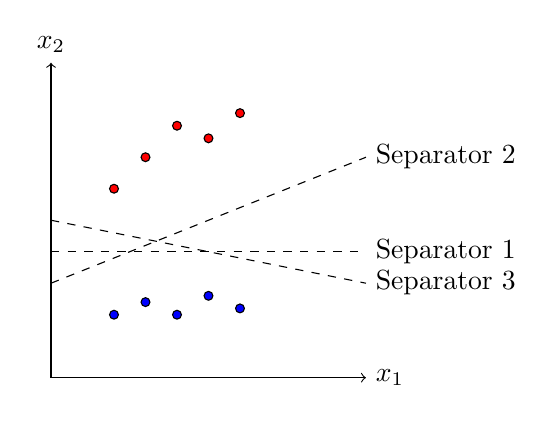
\begin{tikzpicture}[scale=0.8]
    % Coordinate axes
    \draw[->] (0,0) -- (5,0) node[right] {$x_1$};
    \draw[->] (0,0) -- (0,5) node[above] {$x_2$};
    
    % Data points
    \foreach \x/\y in {1/1, 1.5/1.2, 2/1, 2.5/1.3, 3/1.1}
        \draw[fill=blue] (\x,\y) circle (2pt);
    
    \foreach \x/\y in {1/3, 1.5/3.5, 2/4, 2.5/3.8, 3/4.2}
        \draw[fill=red] (\x,\y) circle (2pt);
    
    % Multiple possible decision boundaries
    \draw[dashed] (0,2) -- (5,2) node[right] {Separator 1};
    \draw[dashed] (0,1.5) -- (5,3.5) node[right] {Separator 2};
    \draw[dashed] (0,2.5) -- (5,1.5) node[right] {Separator 3};
\end{tikzpicture}
\caption{Multiple possible linear separators for a linearly separable dataset}
\end{figure}

\section{The Maximum-Margin Approach}

\subsection{The Learning Problem}
Let's formalize the learning problem for linear classification:

Given training data $(\mathbf{x}^{(1)}, y^{(1)}), \ldots, (\mathbf{x}^{(n)}, y^{(n)}) \in \mathbb{R}^d \times \{-1, +1\}$, find $\mathbf{w} \in \mathbb{R}^d$ and $b \in \mathbb{R}$ such that:

\[
y^{(i)}(\mathbf{w} \cdot \mathbf{x}^{(i)} + b) > 0 \quad \text{for all } i = 1, 2, \ldots, n
\]

This condition ensures that all training examples are correctly classified.

\subsection{Scaling the Parameters}
An important observation is that if $(\mathbf{w}, b)$ is a solution to the learning problem, then $(c\mathbf{w}, cb)$ is also a solution for any $c > 0$. This is because:

\[
y^{(i)}(c\mathbf{w} \cdot \mathbf{x}^{(i)} + cb) = c \cdot y^{(i)}(\mathbf{w} \cdot \mathbf{x}^{(i)} + b) > 0
\]

This scaling property allows us to reformulate the problem. We can equivalently ask for:

\[
y^{(i)}(\mathbf{w} \cdot \mathbf{x}^{(i)} + b) \geq 1 \quad \text{for all } i = 1, 2, \ldots, n
\]

This reformulation will be crucial for defining the margin.

\subsection{Defining the Margin}
The margin of a linear classifier is the distance from the decision boundary to the nearest training point. For a linear classifier defined by $\mathbf{w}$ and $b$, the decision boundary is the hyperplane:

\[
\mathbf{w} \cdot \mathbf{x} + b = 0
\]

The constraint $y^{(i)}(\mathbf{w} \cdot \mathbf{x}^{(i)} + b) \geq 1$ implies that:
\begin{itemize}
    \item All positive points ($y^{(i)} = +1$) satisfy $\mathbf{w} \cdot \mathbf{x}^{(i)} + b \geq 1$
    \item All negative points ($y^{(i)} = -1$) satisfy $\mathbf{w} \cdot \mathbf{x}^{(i)} + b \leq -1$
\end{itemize}

This means that all positive points are on or above the hyperplane $\mathbf{w} \cdot \mathbf{x} + b = 1$, and all negative points are on or below the hyperplane $\mathbf{w} \cdot \mathbf{x} + b = -1$.

\begin{figure}[h]
\centering
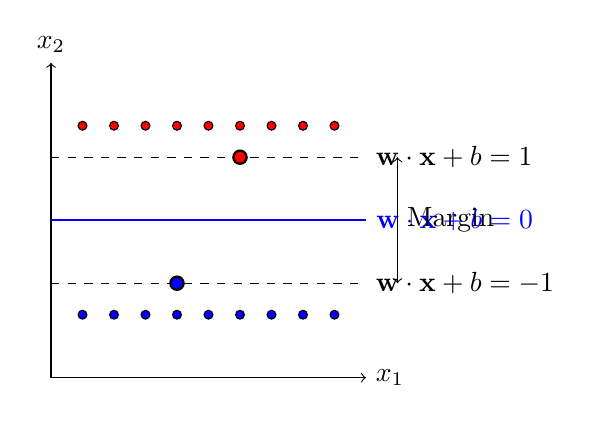
\begin{tikzpicture}[scale=0.8]
    % Coordinate axes
    \draw[->] (0,0) -- (5,0) node[right] {$x_1$};
    \draw[->] (0,0) -- (0,5) node[above] {$x_2$};
    
    % Decision boundary
    \draw[thick, blue] (0,2.5) -- (5,2.5) node[right] {$\mathbf{w} \cdot \mathbf{x} + b = 0$};
    
    % Margin boundaries
    \draw[dashed] (0,1.5) -- (5,1.5) node[right] {$\mathbf{w} \cdot \mathbf{x} + b = -1$};
    \draw[dashed] (0,3.5) -- (5,3.5) node[right] {$\mathbf{w} \cdot \mathbf{x} + b = 1$};
    
    % Margin
    \draw[<->] (5.5,1.5) -- (5.5,3.5) node[midway, right] {Margin};
    
    % Data points
    \foreach \x in {0.5,1,...,4.5}
        \draw[fill=blue] (\x,1) circle (2pt);
    
    \foreach \x in {0.5,1,...,4.5}
        \draw[fill=red] (\x,4) circle (2pt);
    
    % Support vectors
    \draw[fill=blue, thick] (2,1.5) circle (3pt);
    \draw[fill=red, thick] (3,3.5) circle (3pt);
\end{tikzpicture}
\caption{Illustration of the margin in a linearly separable dataset. The support vectors (highlighted) lie exactly on the margin boundaries.}
\end{figure}

\subsection{Calculating the Margin}
The distance from a point $\mathbf{x}$ to the hyperplane $\mathbf{w} \cdot \mathbf{x} + b = 0$ is given by:

\[
\text{distance} = \frac{|\mathbf{w} \cdot \mathbf{x} + b|}{\|\mathbf{w}\|}
\]

For points on the hyperplanes $\mathbf{w} \cdot \mathbf{x} + b = 1$ and $\mathbf{w} \cdot \mathbf{x} + b = -1$, this distance is:

\[
\text{distance} = \frac{1}{\|\mathbf{w}\|}
\]

Therefore, the margin $\gamma$ is:

\[
\gamma = \frac{1}{\|\mathbf{w}\|}
\]

\subsection{Maximizing the Margin}
To maximize the margin $\gamma = \frac{1}{\|\mathbf{w}\|}$, we need to minimize $\|\mathbf{w}\|$. Since minimizing $\|\mathbf{w}\|$ is equivalent to minimizing $\|\mathbf{w}\|^2$ (and the latter is differentiable everywhere), we can formulate the maximum-margin classification problem as:

\[
\min_{\mathbf{w} \in \mathbb{R}^d, b \in \mathbb{R}} \|\mathbf{w}\|^2
\]

subject to:

\[
y^{(i)}(\mathbf{w} \cdot \mathbf{x}^{(i)} + b) \geq 1 \quad \text{for all } i = 1, 2, \ldots, n
\]

This is a convex quadratic optimization problem with linear constraints, which can be solved efficiently using standard optimization techniques.

\section{Support Vector Machines}

\subsection{The Optimization Problem}
The optimization problem for finding the maximum-margin linear classifier is:

\fbox{
\begin{minipage}{\dimexpr\textwidth-2\fboxsep-2\fboxrule\relax}
\textbf{Hard-Margin SVM Optimization Problem}

\begin{align}
\min_{\mathbf{w} \in \mathbb{R}^d, b \in \mathbb{R}} & \|\mathbf{w}\|^2 \\
\text{subject to } & y^{(i)}(\mathbf{w} \cdot \mathbf{x}^{(i)} + b) \geq 1 \quad \text{for all } i = 1, 2, \ldots, n
\end{align}
\end{minipage}
}

This formulation is known as the hard-margin Support Vector Machine (SVM).

\subsection{Properties of the Solution}
The solution to the SVM optimization problem has several important properties:

\begin{itemize}
    \item It is a convex optimization problem, which means that it has a unique global minimum
    \item The solution depends only on a subset of the training points, called support vectors
    \item Support vectors are the points that lie exactly on the margin, i.e., $y^{(i)}(\mathbf{w} \cdot \mathbf{x}^{(i)} + b) = 1$
\end{itemize}

\subsection{Support Vectors}
The solution to the SVM optimization problem can be expressed as:

\[
\mathbf{w} = \sum_{i=1}^{n} \alpha_i y^{(i)} \mathbf{x}^{(i)}
\]

where $\alpha_i \geq 0$ are Lagrange multipliers. Importantly, $\alpha_i > 0$ only for the support vectors (points that lie exactly on the margin). For all other points, $\alpha_i = 0$.

This means that the solution $\mathbf{w}$ is a linear combination of only the support vectors, and the decision boundary is determined entirely by these points.

\begin{figure}[h]
\centering
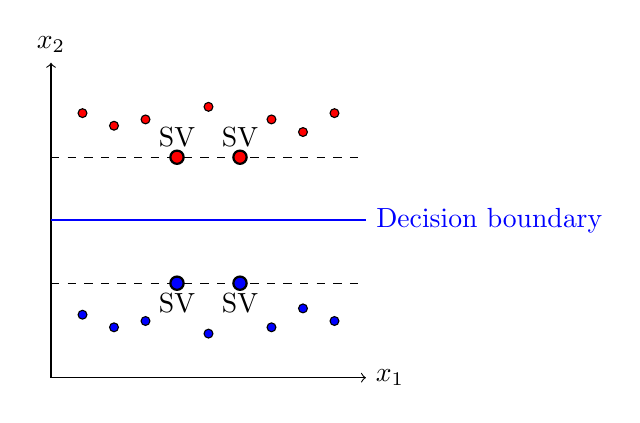
\begin{tikzpicture}[scale=0.8]
    % Coordinate axes
    \draw[->] (0,0) -- (5,0) node[right] {$x_1$};
    \draw[->] (0,0) -- (0,5) node[above] {$x_2$};
    
    % Decision boundary
    \draw[thick, blue] (0,2.5) -- (5,2.5) node[right] {Decision boundary};
    
    % Margin boundaries
    \draw[dashed] (0,1.5) -- (5,1.5);
    \draw[dashed] (0,3.5) -- (5,3.5);
    
    % Data points
    \foreach \x/\y in {0.5/1, 1/0.8, 1.5/0.9, 2.5/0.7, 3.5/0.8, 4/1.1, 4.5/0.9}
        \draw[fill=blue] (\x,\y) circle (2pt);
    
    \foreach \x/\y in {0.5/4.2, 1/4, 1.5/4.1, 2.5/4.3, 3.5/4.1, 4/3.9, 4.5/4.2}
        \draw[fill=red] (\x,\y) circle (2pt);
    
    % Support vectors
    \draw[fill=blue, thick] (2,1.5) circle (3pt) node[below] {SV};
    \draw[fill=blue, thick] (3,1.5) circle (3pt) node[below] {SV};
    \draw[fill=red, thick] (2,3.5) circle (3pt) node[above] {SV};
    \draw[fill=red, thick] (3,3.5) circle (3pt) node[above] {SV};
\end{tikzpicture}
\caption{Support vectors (SV) are the points that lie exactly on the margin boundaries. The decision boundary is determined entirely by these points.}
\end{figure}

\section{The Dual Formulation}

\subsection{Lagrangian Formulation}
To solve the SVM optimization problem, we can use Lagrange multipliers. The Lagrangian is:

\[
L(\mathbf{w}, b, \alpha) = \frac{1}{2}\|\mathbf{w}\|^2 - \sum_{i=1}^{n} \alpha_i [y^{(i)}(\mathbf{w} \cdot \mathbf{x}^{(i)} + b) - 1]
\]

where $\alpha_i \geq 0$ are the Lagrange multipliers.

\subsection{Dual Problem}
By taking derivatives of the Lagrangian with respect to $\mathbf{w}$ and $b$ and setting them to zero, we get:

\[
\mathbf{w} = \sum_{i=1}^{n} \alpha_i y^{(i)} \mathbf{x}^{(i)}
\]

\[
\sum_{i=1}^{n} \alpha_i y^{(i)} = 0
\]

Substituting these back into the Lagrangian, we get the dual problem:

\[
\max_{\alpha} \sum_{i=1}^{n} \alpha_i - \frac{1}{2} \sum_{i=1}^{n} \sum_{j=1}^{n} \alpha_i \alpha_j y^{(i)} y^{(j)} \mathbf{x}^{(i)} \cdot \mathbf{x}^{(j)}
\]

subject to:

\[
\alpha_i \geq 0 \quad \text{for all } i = 1, 2, \ldots, n
\]

\[
\sum_{i=1}^{n} \alpha_i y^{(i)} = 0
\]

This dual formulation is often easier to solve than the primal problem, especially when the number of features is large.

\section{Example: Iris Dataset}

\subsection{Dataset Description}
The Iris dataset is a classic dataset in machine learning, collected by the botanist Edgar Anderson and made famous by the statistician Ronald Fisher. It contains measurements of 150 iris flowers from three different species:

\begin{itemize}
    \item Iris setosa
    \item Iris versicolor
    \item Iris virginica
\end{itemize}

For each flower, four measurements were taken:
\begin{itemize}
    \item Sepal length
    \item Sepal width
    \item Petal length
    \item Petal width
\end{itemize}

\subsection{Binary Classification Example}
For simplicity, let's consider a binary classification problem using only two of the species (setosa and versicolor) and two of the features (sepal width and petal width).

\begin{figure}[h]
\centering
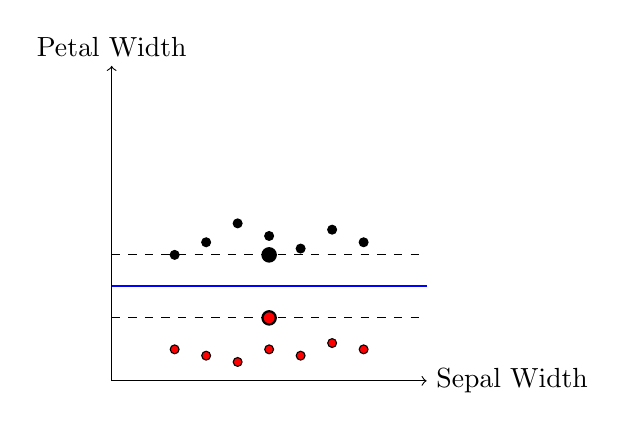
\begin{tikzpicture}[scale=0.8]
    % Coordinate axes
    \draw[->] (0,0) -- (5,0) node[right] {Sepal Width};
    \draw[->] (0,0) -- (0,5) node[above] {Petal Width};
    
    % Setosa (red circles)
    \foreach \x/\y in {1/0.5, 1.5/0.4, 2/0.3, 2.5/0.5, 3/0.4, 3.5/0.6, 4/0.5}
        \draw[fill=red] (\x,\y) circle (2pt);
    
    % Versicolor (black triangles)
    \foreach \x/\y in {1/2, 1.5/2.2, 2/2.5, 2.5/2.3, 3/2.1, 3.5/2.4, 4/2.2}
        \draw[fill=black] (\x,\y) circle (2pt);
    
    % Decision boundary
    \draw[thick, blue] (0,1.5) -- (5,1.5);
    
    % Margin boundaries
    \draw[dashed] (0,1) -- (5,1);
    \draw[dashed] (0,2) -- (5,2);
    
    % Support vectors
    \draw[fill=red, thick] (2.5,1) circle (3pt);
    \draw[fill=black, thick] (2.5,2) circle (3pt);
\end{tikzpicture}
\caption{SVM classification of Iris setosa (red circles) and Iris versicolor (black triangles) using sepal width and petal width features.}
\end{figure}

In this example, the data is linearly separable, and the SVM finds the maximum-margin linear classifier. The support vectors are the points that lie exactly on the margin boundaries.

\section{Soft-Margin SVM}

\subsection{Handling Non-linearly Separable Data}
The hard-margin SVM assumes that the data is linearly separable. However, in real-world scenarios, data is often not perfectly separable due to noise or outliers. To handle such cases, we can use a soft-margin SVM, which allows for some misclassifications.

\subsection{Slack Variables}
We introduce slack variables $\xi_i \geq 0$ for each training point, which measure the degree of misclassification:

\[
y^{(i)}(\mathbf{w} \cdot \mathbf{x}^{(i)} + b) \geq 1 - \xi_i \quad \text{for all } i = 1, 2, \ldots, n
\]

If $\xi_i = 0$, the point is correctly classified and on or beyond the margin.
If $0 < \xi_i \leq 1$, the point is correctly classified but within the margin.
If $\xi_i > 1$, the point is misclassified.

\subsection{Optimization Problem}
The soft-margin SVM optimization problem is:

\fbox{
\begin{minipage}{\dimexpr\textwidth-2\fboxsep-2\fboxrule\relax}
\textbf{Soft-Margin SVM Optimization Problem}

\begin{align}
\min_{\mathbf{w}, b, \xi} & \frac{1}{2}\|\mathbf{w}\|^2 + C \sum_{i=1}^{n} \xi_i \\
\text{subject to } & y^{(i)}(\mathbf{w} \cdot \mathbf{x}^{(i)} + b) \geq 1 - \xi_i \quad \text{for all } i = 1, 2, \ldots, n \\
& \xi_i \geq 0 \quad \text{for all } i = 1, 2, \ldots, n
\end{align}
\end{minipage}
}

The parameter $C > 0$ controls the trade-off between maximizing the margin and minimizing the classification error. A larger $C$ places more emphasis on correctly classifying all training points, while a smaller $C$ places more emphasis on maximizing the margin.

\begin{figure}[h]
\centering
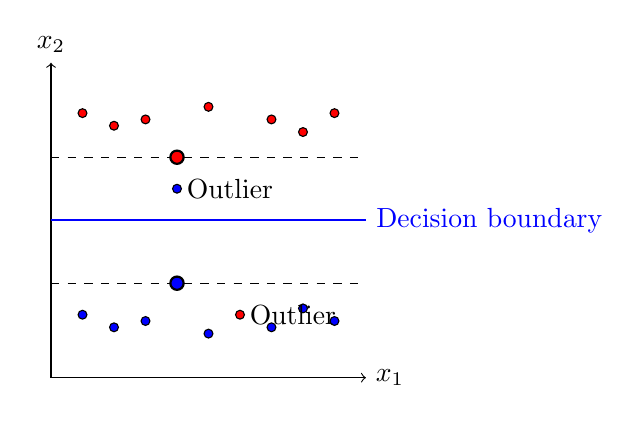
\begin{tikzpicture}[scale=0.8]
    % Coordinate axes
    \draw[->] (0,0) -- (5,0) node[right] {$x_1$};
    \draw[->] (0,0) -- (0,5) node[above] {$x_2$};
    
    % Decision boundary
    \draw[thick, blue] (0,2.5) -- (5,2.5) node[right] {Decision boundary};
    
    % Margin boundaries
    \draw[dashed] (0,1.5) -- (5,1.5);
    \draw[dashed] (0,3.5) -- (5,3.5);
    
    % Data points
    \foreach \x/\y in {0.5/1, 1/0.8, 1.5/0.9, 2.5/0.7, 3.5/0.8, 4/1.1, 4.5/0.9}
        \draw[fill=blue] (\x,\y) circle (2pt);
    
    \foreach \x/\y in {0.5/4.2, 1/4, 1.5/4.1, 2.5/4.3, 3.5/4.1, 4/3.9, 4.5/4.2}
        \draw[fill=red] (\x,\y) circle (2pt);
    
    % Outliers
    \draw[fill=blue] (2,3) circle (2pt) node[right] {Outlier};
    \draw[fill=red] (3,1) circle (2pt) node[right] {Outlier};
    
    % Support vectors
    \draw[fill=blue, thick] (2,1.5) circle (3pt);
    \draw[fill=red, thick] (2,3.5) circle (3pt);
\end{tikzpicture}
\caption{Soft-margin SVM allows for some misclassifications to handle outliers or non-linearly separable data.}
\end{figure}

\section{Kernel Methods for Non-linear Classification}

\subsection{Limitations of Linear Classifiers}
Linear classifiers, including hard-margin and soft-margin SVMs, can only learn linear decision boundaries. However, many real-world datasets require non-linear decision boundaries for effective classification.

\begin{figure}[h]
\centering
\begin{tikzpicture}[scale=0.8]
    % Coordinate axes
    \draw[->] (0,0) -- (5,0) node[right] {$x_1$};
    \draw[->] (0,0) -- (0,5) node[above] {$x_2$};
    
    % Data points - XOR pattern
    \draw[fill=red] (1,1) circle (2pt);
    \draw[fill=red] (4,4) circle (2pt);
    \draw[fill=blue] (1,4) circle (2pt);
    \draw[fill=blue] (4,1) circle (2pt);
    
    % Non-linear decision boundary
    \draw[thick, blue] (2.5,0) arc (0:180:2.5);
    \draw[thick, blue] (2.5,0) arc (0:180:2.5 and 1.25);
    \draw[thick, blue] (2.5,5) arc (180:360:2.5 and 1.25);
\end{tikzpicture}
\caption{Example of data that requires a non-linear decision boundary (XOR pattern)}
\end{figure}

\subsection{The Kernel Trick}
The kernel trick is a clever technique that allows SVMs to learn non-linear decision boundaries without explicitly mapping the data to a higher-dimensional space. It relies on the observation that the dual formulation of the SVM optimization problem only depends on inner products between data points.

\subsubsection{Feature Maps}
Let $\phi: \mathbb{R}^d \rightarrow \mathbb{R}^D$ be a feature map that maps data from the original $d$-dimensional space to a higher-dimensional space $\mathbb{R}^D$. The idea is to find a linear boundary in this higher-dimensional space, which corresponds to a non-linear boundary in the original space.

\subsubsection{Kernel Functions}
A kernel function $K: \mathbb{R}^d \times \mathbb{R}^d \rightarrow \mathbb{R}$ computes the inner product in the higher-dimensional space without explicitly computing the mapping:

\[
K(\mathbf{x}, \mathbf{z}) = \phi(\mathbf{x}) \cdot \phi(\mathbf{z})
\]

This is powerful because:
\begin{itemize}
    \item We never need to explicitly compute $\phi(\mathbf{x})$, which could be very high-dimensional or even infinite-dimensional
    \item We only need to define the kernel function $K$, which computes the inner product directly
\end{itemize}

\subsection{Common Kernel Functions}
Several kernel functions are commonly used in practice:

\begin{itemize}
    \item \textbf{Linear kernel}: $K(\mathbf{x}, \mathbf{z}) = \mathbf{x} \cdot \mathbf{z}$
    \item \textbf{Polynomial kernel}: $K(\mathbf{x}, \mathbf{z}) = (\mathbf{x} \cdot \mathbf{z} + c)^d$, where $c \geq 0$ and $d \in \mathbb{N}$
    \item \textbf{Radial Basis Function (RBF) kernel}: $K(\mathbf{x}, \mathbf{z}) = \exp(-\gamma \|\mathbf{x} - \mathbf{z}\|^2)$, where $\gamma > 0$
    \item \textbf{Sigmoid kernel}: $K(\mathbf{x}, \mathbf{z}) = \tanh(\alpha \mathbf{x} \cdot \mathbf{z} + c)$, where $\alpha > 0$ and $c \geq 0$
\end{itemize}

\subsection{Kernel SVM Formulation}
The dual formulation of the SVM optimization problem with kernels is:

\[
\max_{\alpha} \sum_{i=1}^{n} \alpha_i - \frac{1}{2} \sum_{i=1}^{n} \sum_{j=1}^{n} \alpha_i \alpha_j y^{(i)} y^{(j)} K(\mathbf{x}^{(i)}, \mathbf{x}^{(j)})
\]

subject to:

\[
\alpha_i \geq 0 \quad \text{for all } i = 1, 2, \ldots, n
\]

\[
\sum_{i=1}^{n} \alpha_i y^{(i)} = 0
\]

The decision function becomes:

\[
f(\mathbf{x}) = \text{sign}\left(\sum_{i=1}^{n} \alpha_i y^{(i)} K(\mathbf{x}^{(i)}, \mathbf{x}) + b\right)
\]

\subsection{Example: RBF Kernel}
The RBF kernel is particularly popular because it can model complex non-linear decision boundaries. It effectively measures the similarity between two points based on their Euclidean distance:

\[
K(\mathbf{x}, \mathbf{z}) = \exp(-\gamma \|\mathbf{x} - \mathbf{z}\|^2)
\]

The parameter $\gamma$ controls the "width" of the kernel:
\begin{itemize}
    \item Small $\gamma$: Wide kernel, smooth decision boundary
    \item Large $\gamma$: Narrow kernel, more complex decision boundary
\end{itemize}

\begin{figure}[h]
\centering
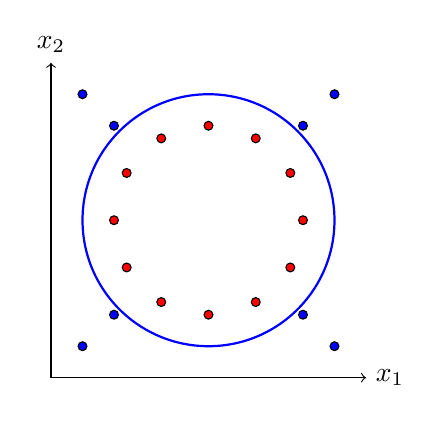
\begin{tikzpicture}[scale=0.8]
    % Coordinate axes
    \draw[->] (0,0) -- (5,0) node[right] {$x_1$};
    \draw[->] (0,0) -- (0,5) node[above] {$x_2$};
    
    % Data points - circular pattern
    \foreach \angle in {0,30,...,330}
        \draw[fill=red] ({2.5+1.5*cos(\angle)},{2.5+1.5*sin(\angle)}) circle (2pt);
    
    \foreach \x/\y in {0.5/0.5, 0.5/4.5, 4.5/0.5, 4.5/4.5, 1/1, 1/4, 4/1, 4/4}
        \draw[fill=blue] (\x,\y) circle (2pt);
    
    % Non-linear decision boundary
    \draw[thick, blue] (2.5,2.5) circle (2);
\end{tikzpicture}
\caption{Example of a non-linear decision boundary learned using an RBF kernel}
\end{figure}

\section{Multi-class SVMs}

\subsection{Extending SVMs to Multiple Classes}
SVMs are inherently binary classifiers, but many real-world problems involve multiple classes. Several strategies exist for extending SVMs to multi-class classification:

\subsubsection{One-vs-Rest (OVR)}
In the One-vs-Rest approach:
\begin{itemize}
    \item Train $k$ binary SVMs, where $k$ is the number of classes
    \item Each SVM distinguishes one class from all other classes
    \item For a new point, evaluate all $k$ SVMs and assign the class with the highest confidence score
\end{itemize}

\begin{figure}[h]
\centering
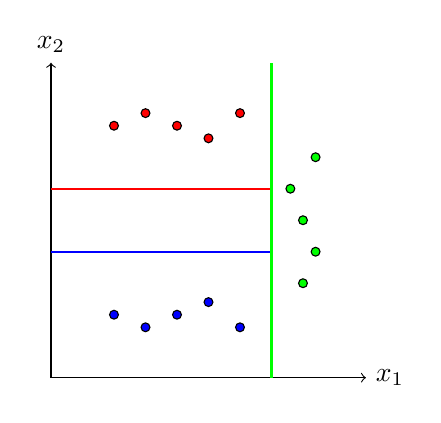
\begin{tikzpicture}[scale=0.8]
    % Coordinate axes
    \draw[->] (0,0) -- (5,0) node[right] {$x_1$};
    \draw[->] (0,0) -- (0,5) node[above] {$x_2$};
    
    % Class 1 (red)
    \foreach \x/\y in {1/4, 1.5/4.2, 2/4, 2.5/3.8, 3/4.2}
        \draw[fill=red] (\x,\y) circle (2pt);
    
    % Class 2 (blue)
    \foreach \x/\y in {1/1, 1.5/0.8, 2/1, 2.5/1.2, 3/0.8}
        \draw[fill=blue] (\x,\y) circle (2pt);
    
    % Class 3 (green)
    \foreach \x/\y in {4/2.5, 4.2/2, 4/1.5, 3.8/3, 4.2/3.5}
        \draw[fill=green] (\x,\y) circle (2pt);
    
    % Decision boundaries
    \draw[thick, red] (0,3) -- (3.5,3) -- (3.5,5);
    \draw[thick, blue] (0,2) -- (3.5,2) -- (3.5,0);
    \draw[thick, green] (3.5,0) -- (3.5,5);
\end{tikzpicture}
\caption{One-vs-Rest approach for multi-class SVM with three classes}
\end{figure}

\subsubsection{One-vs-One (OVO)}
In the One-vs-One approach:
\begin{itemize}
    \item Train $\binom{k}{2} = \frac{k(k-1)}{2}$ binary SVMs, one for each pair of classes
    \item For a new point, each binary SVM votes for one class
    \item Assign the class with the most votes
\end{itemize}

\begin{figure}[h]
\centering
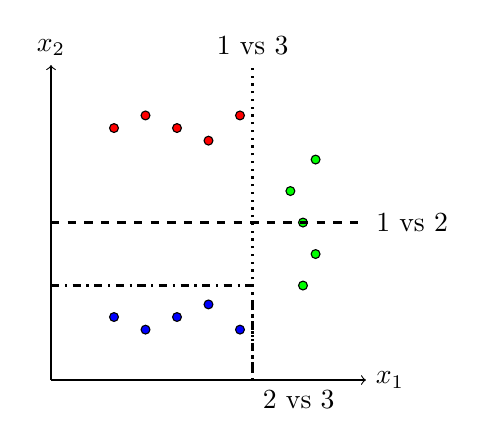
\begin{tikzpicture}[scale=0.8]
    % Coordinate axes
    \draw[->] (0,0) -- (5,0) node[right] {$x_1$};
    \draw[->] (0,0) -- (0,5) node[above] {$x_2$};
    
    % Class 1 (red)
    \foreach \x/\y in {1/4, 1.5/4.2, 2/4, 2.5/3.8, 3/4.2}
        \draw[fill=red] (\x,\y) circle (2pt);
    
    % Class 2 (blue)
    \foreach \x/\y in {1/1, 1.5/0.8, 2/1, 2.5/1.2, 3/0.8}
        \draw[fill=blue] (\x,\y) circle (2pt);
    
    % Class 3 (green)
    \foreach \x/\y in {4/2.5, 4.2/2, 4/1.5, 3.8/3, 4.2/3.5}
        \draw[fill=green] (\x,\y) circle (2pt);
    
    % Decision boundaries
    \draw[thick, dashed] (0,2.5) -- (5,2.5) node[right] {1 vs 2};
    \draw[thick, dotted] (3.2,0) -- (3.2,5) node[above] {1 vs 3};
    \draw[thick, dashdotted] (0,1.5) -- (3.2,1.5) -- (3.2,0) node[below right] {2 vs 3};
\end{tikzpicture}
\caption{One-vs-One approach for multi-class SVM with three classes}
\end{figure}

\subsubsection{Direct Multi-class Formulation}
There are also direct formulations of multi-class SVMs that solve a single optimization problem:
\begin{itemize}
    \item Crammer and Singer's multi-class SVM
    \item Weston and Watkins' multi-class SVM
\end{itemize}

These formulations are more complex but can sometimes yield better results than the OVR or OVO approaches.

\subsection{Comparison of Multi-class Strategies}
\begin{itemize}
    \item \textbf{One-vs-Rest}:
    \begin{itemize}
        \item Pros: Simple, only requires $k$ classifiers
        \item Cons: Class imbalance, ambiguous regions
    \end{itemize}
    \item \textbf{One-vs-One}:
    \begin{itemize}
        \item Pros: Better handling of class imbalance, smaller training sets for each classifier
        \item Cons: Requires $\binom{k}{2}$ classifiers, which can be large for many classes
    \end{itemize}
    \item \textbf{Direct Multi-class}:
    \begin{itemize}
        \item Pros: Theoretically more principled, considers all classes simultaneously
        \item Cons: More complex optimization problem, computationally expensive
    \end{itemize}
\end{itemize}

\section{Practical Considerations}

\subsection{Hyperparameter Selection}
SVMs have several hyperparameters that need to be tuned:
\begin{itemize}
    \item $C$: The regularization parameter in soft-margin SVMs
    \item Kernel parameters (e.g., $\gamma$ in RBF kernel, $d$ in polynomial kernel)
\end{itemize}

These hyperparameters are typically selected using cross-validation:
\begin{itemize}
    \item Split the data into training and validation sets
    \item Train SVMs with different hyperparameter values on the training set
    \item Evaluate performance on the validation set
    \item Select the hyperparameters that yield the best validation performance
\end{itemize}

\subsection{Feature Scaling}
SVMs are sensitive to the scale of the features. It's generally recommended to scale the features before training an SVM:
\begin{itemize}
    \item Standardization: $x' = \frac{x - \mu}{\sigma}$
    \item Min-max scaling: $x' = \frac{x - \min(x)}{\max(x) - \min(x)}$
\end{itemize}

\subsection{Handling Large Datasets}
Standard SVM implementations have time complexity $O(n^2)$ to $O(n^3)$, where $n$ is the number of training examples. This can be prohibitive for large datasets. Several approaches exist for scaling SVMs to large datasets:
\begin{itemize}
    \item Chunking: Solve the optimization problem in smaller chunks
    \item Sequential Minimal Optimization (SMO): Optimize two Lagrange multipliers at a time
    \item Stochastic gradient descent: Approximate the SVM solution using SGD
    \item Linear SVMs: For linear kernels, specialized algorithms like LIBLINEAR can scale to millions of examples
\end{itemize}

\subsection{Probabilistic Outputs}
Standard SVMs output only the class label, not a probability. However, there are methods to convert SVM outputs to probabilities:
\begin{itemize}
    \item Platt scaling: Fit a logistic regression model to the SVM scores
    \item Isotonic regression: A more flexible non-parametric approach
\end{itemize}

\section{Worked Examples}

\subsection{Example 1: Linear SVM on a 2D Dataset}
Consider a simple 2D dataset with two classes:
\begin{itemize}
    \item Positive examples: $(1,1)$, $(2,3)$, $(3,2)$
    \item Negative examples: $(1,3)$, $(2,1)$, $(3,3)$
\end{itemize}

\begin{figure}[h]
\centering
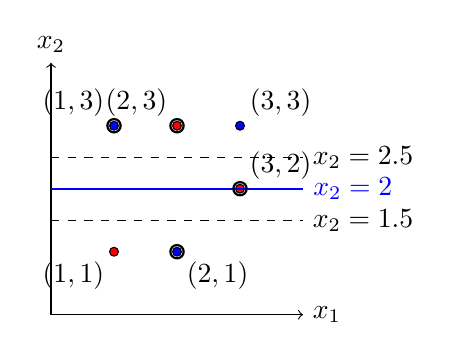
\begin{tikzpicture}[scale=0.8]
    % Coordinate axes
    \draw[->] (0,0) -- (4,0) node[right] {$x_1$};
    \draw[->] (0,0) -- (0,4) node[above] {$x_2$};
    
    % Data points
    \draw[fill=red] (1,1) circle (2pt) node[below left] {$(1,1)$};
    \draw[fill=red] (2,3) circle (2pt) node[above left] {$(2,3)$};
    \draw[fill=red] (3,2) circle (2pt) node[above right] {$(3,2)$};
    \draw[fill=blue] (1,3) circle (2pt) node[above left] {$(1,3)$};
    \draw[fill=blue] (2,1) circle (2pt) node[below right] {$(2,1)$};
    \draw[fill=blue] (3,3) circle (2pt) node[above right] {$(3,3)$};
    
    % Decision boundary
    \draw[thick, blue] (0,2) -- (4,2) node[right] {$x_2 = 2$};
    
    % Margin boundaries
    \draw[dashed] (0,1.5) -- (4,1.5) node[right] {$x_2 = 1.5$};
    \draw[dashed] (0,2.5) -- (4,2.5) node[right] {$x_2 = 2.5$};
    
    % Support vectors
    \draw[thick] (2,1) circle (3pt);
    \draw[thick] (3,2) circle (3pt);
    \draw[thick] (1,3) circle (3pt);
    \draw[thick] (2,3) circle (3pt);
\end{tikzpicture}
\caption{Linear SVM on a 2D dataset. The decision boundary is $x_2 = 2$, and the support vectors are circled.}
\end{figure}

The SVM finds the decision boundary $x_2 = 2$, which corresponds to $w = (0, 1)$ and $b = -2$. The margin is $\gamma = 1/\|w\| = 1$, and the support vectors are the points closest to the decision boundary: $(2,1)$, $(3,2)$, $(1,3)$, and $(2,3)$.

\subsection{Example 2: Soft-Margin SVM with Outliers}
Now, let's add an outlier to the dataset:
\begin{itemize}
    \item Positive examples: $(1,1)$, $(2,3)$, $(3,2)$, $(2,0.5)$ (outlier)
    \item Negative examples: $(1,3)$, $(2,1)$, $(3,3)$
\end{itemize}

\begin{figure}[h]
\centering
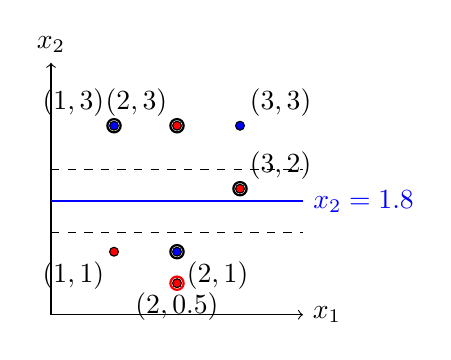
\begin{tikzpicture}[scale=0.8]
    % Coordinate axes
    \draw[->] (0,0) -- (4,0) node[right] {$x_1$};
    \draw[->] (0,0) -- (0,4) node[above] {$x_2$};
    
    % Data points
    \draw[fill=red] (1,1) circle (2pt) node[below left] {$(1,1)$};
    \draw[fill=red] (2,3) circle (2pt) node[above left] {$(2,3)$};
    \draw[fill=red] (3,2) circle (2pt) node[above right] {$(3,2)$};
    \draw[fill=red] (2,0.5) circle (2pt) node[below] {$(2,0.5)$};
    \draw[fill=blue] (1,3) circle (2pt) node[above left] {$(1,3)$};
    \draw[fill=blue] (2,1) circle (2pt) node[below right] {$(2,1)$};
    \draw[fill=blue] (3,3) circle (2pt) node[above right] {$(3,3)$};
    
    % Decision boundary
    \draw[thick, blue] (0,1.8) -- (4,1.8) node[right] {$x_2 = 1.8$};
    
    % Margin boundaries
    \draw[dashed] (0,1.3) -- (4,1.3);
    \draw[dashed] (0,2.3) -- (4,2.3);
    
    % Support vectors
    \draw[thick] (2,1) circle (3pt);
    \draw[thick] (3,2) circle (3pt);
    \draw[thick] (1,3) circle (3pt);
    \draw[thick] (2,3) circle (3pt);
    
    % Outlier
    \draw[thick, red] (2,0.5) circle (3pt);
\end{tikzpicture}
\caption{Soft-margin SVM with an outlier. The decision boundary shifts slightly to accommodate the outlier.}
\end{figure}

With a hard-margin SVM, this dataset would not be linearly separable due to the outlier. However, a soft-margin SVM can handle the outlier by allowing it to be misclassified (with a penalty determined by the parameter $C$).

\subsection{Example 3: Non-linear SVM with RBF Kernel}
Consider a dataset with a circular pattern:
\begin{itemize}
    \item Positive examples: Points inside a circle
    \item Negative examples: Points outside the circle
\end{itemize}

\begin{figure}[h]
\centering
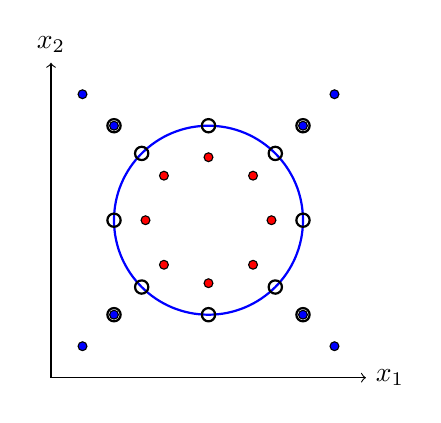
\begin{tikzpicture}[scale=0.8]
    % Coordinate axes
    \draw[->] (0,0) -- (5,0) node[right] {$x_1$};
    \draw[->] (0,0) -- (0,5) node[above] {$x_2$};
    
    % Circle
    \draw[thick, blue] (2.5,2.5) circle (1.5);
    
    % Points inside the circle (positive)
    \foreach \angle in {0,45,...,315}
        \draw[fill=red] ({2.5+cos(\angle)},{2.5+sin(\angle)}) circle (2pt);
    
    % Points outside the circle (negative)
    \foreach \x/\y in {0.5/0.5, 0.5/4.5, 4.5/0.5, 4.5/4.5, 1/1, 1/4, 4/1, 4/4}
        \draw[fill=blue] (\x,\y) circle (2pt);
    
    % Support vectors
    \foreach \angle in {0,45,...,315}
        \draw[thick] ({2.5+1.5*cos(\angle)},{2.5+1.5*sin(\angle)}) circle (3pt);
    
    \foreach \x/\y in {1/1, 1/4, 4/1, 4/4}
        \draw[thick] (\x,\y) circle (3pt);
\end{tikzpicture}
\caption{Non-linear SVM with RBF kernel. The decision boundary is a circle, and the support vectors are circled.}
\end{figure}

This dataset is not linearly separable, but an SVM with an RBF kernel can learn the circular decision boundary. The support vectors are the points closest to the decision boundary.

\section{Summary and Key Takeaways}

\subsection{Core Concepts}
\begin{itemize}
    \item Support Vector Machines (SVMs) find the linear classifier with the maximum margin between classes
    \item The margin is the distance from the decision boundary to the nearest training points
    \item Maximizing the margin leads to better generalization to unseen data
    \item The optimization problem for hard-margin SVMs is to minimize $\|w\|^2$ subject to $y^{(i)}(w \cdot x^{(i)} + b) \geq 1$ for all training points
\end{itemize}

\subsection{Extensions}
\begin{itemize}
    \item Soft-margin SVMs allow for some misclassifications to handle non-linearly separable data
    \item Kernel SVMs use the kernel trick to learn non-linear decision boundaries
    \item Multi-class SVMs extend binary SVMs to handle multiple classes
\end{itemize}

\subsection{Strengths of SVMs}
\begin{itemize}
    \item Effective in high-dimensional spaces
    \item Memory efficient (only support vectors are needed for prediction)
    \item Versatile (different kernel functions for different types of data)
    \item Robust to overfitting, especially in high-dimensional spaces
\end{itemize}

\subsection{Limitations of SVMs}
\begin{itemize}
    \item Computationally intensive for large datasets
    \item Sensitive to the choice of kernel and hyperparameters
    \item No direct probability estimates (though methods exist to convert scores to probabilities)
    \item Can be challenging to interpret, especially with non-linear kernels
\end{itemize}

\subsection{Practical Tips}
\begin{itemize}
    \item Scale features before training SVMs
    \item Use cross-validation to select hyperparameters
    \item Start with a linear kernel and move to more complex kernels if needed
    \item For large datasets, consider specialized implementations or approximations
\end{itemize}

\subsection{Connections to Other Methods}
\begin{itemize}
    \item SVMs are related to logistic regression, but focus on the margin rather than probabilistic interpretation
    \item The kernel trick used in SVMs is also applicable to other methods (e.g., kernel PCA, kernel k-means)
    \item SVMs can be viewed as a special case of regularized empirical risk minimization
    \item The concept of maximum margin has influenced other methods, such as boosting algorithms
\end{itemize}

\end{document}\documentclass{article}
\usepackage{amsmath, amssymb, graphicx, geometry, tikz, array, booktabs, enumitem, listings, xcolor, fancyhdr, float, subcaption, hyperref}

\title{Module 6: SVM Example - Parameter Selection and Sentiment Analysis}
\author{Machine Learning Course}
\date{}

\begin{document}

\maketitle
\tableofcontents
\newpage

\section{Introduction to SVM Parameter Selection}

\subsection{The Importance of Parameter Tuning}
Support Vector Machines (SVMs) are powerful classification algorithms that find the optimal hyperplane to separate data points of different classes. However, their performance heavily depends on the proper selection of hyperparameters, particularly the regularization parameter $C$. This document explores a practical example of applying SVMs to sentiment analysis and demonstrates the critical role of parameter tuning in achieving optimal performance.

\subsection{Review of the Soft-Margin SVM}
Before diving into the example, let's briefly review the soft-margin SVM formulation:

\fbox{
\begin{minipage}{\dimexpr\textwidth-2\fboxsep-2\fboxrule\relax}
\textbf{Soft-Margin SVM Optimization Problem}

\begin{align}
\min_{w\in\mathbb{R}^{d},b\in\mathbb{R},\xi\in\mathbb{R}^{n}} & \|w\|^{2}+C\sum_{i=1}^{n}\xi_{i} \\
\text{subject to: } & y^{(i)}(w\cdot x^{(i)}+b)\geq 1-\xi_{i} \text{ for all } i=1,2,...,n \\
& \xi_i \geq 0 \text{ for all } i=1,2,...,n
\end{align}
\end{minipage}
}

The soft-margin SVM introduces slack variables $\xi_i$ that allow for some misclassifications in the training data. The parameter $C$ controls the trade-off between maximizing the margin (minimizing $\|w\|^2$) and minimizing the classification error (minimizing $\sum_{i=1}^{n}\xi_{i}$).

\section{Understanding the Regularization Parameter $C$}

\subsection{The Role of Parameter $C$}
The parameter $C$ in the soft-margin SVM formulation serves as a regularization parameter that controls the trade-off between two competing objectives:

\begin{itemize}
    \item \textbf{Maximizing the margin}: Achieved by minimizing $\|w\|^2$
    \item \textbf{Minimizing training errors}: Achieved by minimizing $\sum_{i=1}^{n}\xi_{i}$
\end{itemize}

The value of $C$ determines the relative importance of these objectives:

\begin{itemize}
    \item \textbf{Small $C$}: Places more emphasis on maximizing the margin, even if it means allowing more training errors
    \item \textbf{Large $C$}: Places more emphasis on minimizing training errors, potentially at the cost of a smaller margin
\end{itemize}

\subsection{Geometric Interpretation}
The parameter $C$ affects the geometry of the decision boundary:

\begin{figure}[h]
\centering
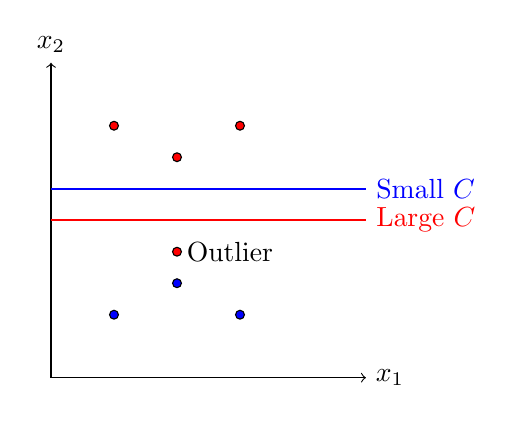
\begin{tikzpicture}[scale=0.8]
    % Coordinate axes
    \draw[->] (0,0) -- (5,0) node[right] {$x_1$};
    \draw[->] (0,0) -- (0,5) node[above] {$x_2$};
    
    % Data points
    \draw[fill=red] (1,4) circle (2pt);
    \draw[fill=red] (2,3.5) circle (2pt);
    \draw[fill=red] (3,4) circle (2pt);
    \draw[fill=blue] (1,1) circle (2pt);
    \draw[fill=blue] (2,1.5) circle (2pt);
    \draw[fill=blue] (3,1) circle (2pt);
    
    % Outlier
    \draw[fill=red] (2,2) circle (2pt) node[right] {Outlier};
    
    % Decision boundaries
    \draw[thick, blue] (0,3) -- (5,3) node[right] {Small $C$};
    \draw[thick, red] (0,2.5) -- (5,2.5) node[right] {Large $C$};
\end{tikzpicture}
\caption{Effect of parameter $C$ on the decision boundary. A small $C$ (blue line) allows the outlier to be misclassified to maintain a larger margin. A large $C$ (red line) adjusts the boundary to correctly classify the outlier, resulting in a smaller margin.}
\end{figure}

\subsection{Practical Implications}
The choice of $C$ has significant practical implications:

\begin{itemize}
    \item \textbf{Overfitting vs. Underfitting}: Large $C$ values can lead to overfitting, while small $C$ values might result in underfitting
    \item \textbf{Number of Support Vectors}: Larger $C$ values typically result in fewer support vectors
    \item \textbf{Generalization Performance}: The optimal $C$ value balances training accuracy and generalization to unseen data
\end{itemize}

\section{Sentiment Analysis Case Study}

\subsection{Dataset Description}
The case study uses a sentiment analysis dataset with the following characteristics:

\begin{itemize}
    \item \textbf{Source}: Reviews from Amazon, Yelp, and IMDB
    \item \textbf{Labels}: Binary classification (positive or negative sentiment)
    \item \textbf{Representation}: Bag-of-words with a vocabulary of 4500 words
    \item \textbf{Size}: 2500 training sentences, 500 test sentences
\end{itemize}

\subsection{Example Sentences}
The dataset contains sentences like:

\begin{itemize}
    \item "Needless to say, I wasted my money." (Negative)
    \item "He was very impressed when going from the original battery to the extended battery." (Positive)
    \item "I have to jiggle the plug to get it to line up right to get decent volume." (Negative)
    \item "Will order from them again!" (Positive)
\end{itemize}

\subsection{Feature Representation}
The bag-of-words representation transforms each sentence into a high-dimensional vector:

\begin{itemize}
    \item Each dimension corresponds to a word in the vocabulary
    \item The value in each dimension represents the presence or frequency of the word in the sentence
    \item This creates a sparse vector representation (most entries are zero)
\end{itemize}

\begin{figure}[h]
\centering
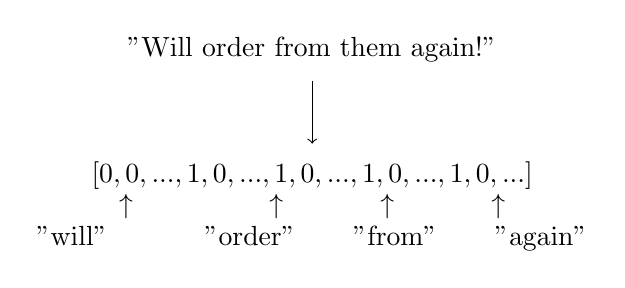
\begin{tikzpicture}[scale=0.8]
    % Sentence
    \node[align=left] at (0,4) {"Will order from them again!"};
    
    % Arrow
    \draw[->] (0,3.5) -- (0,2.5);
    
    % Vector representation
    \node[align=left] at (0,2) {$[0, 0, ..., 1, 0, ..., 1, 0, ..., 1, 0, ..., 1, 0, ...]$};
    \node[align=left] at (0,1.5) {$\uparrow$ \hspace{1.5cm} $\uparrow$ \hspace{1cm} $\uparrow$ \hspace{1cm} $\uparrow$};
    \node[align=left] at (0,1) {"will" \hspace{1cm} "order" \hspace{0.5cm} "from" \hspace{0.5cm} "again"};
\end{tikzpicture}
\caption{Bag-of-words representation of a sentence. Each word in the vocabulary corresponds to a dimension in the feature vector.}
\end{figure}

\section{Parameter Selection through Cross-Validation}

\subsection{The Cross-Validation Procedure}
To find the optimal value of $C$, the study employs 5-fold cross-validation:

\begin{enumerate}
    \item Divide the training data into 5 equal folds
    \item For each value of $C$:
    \begin{enumerate}
        \item For each fold $i$ (from 1 to 5):
        \begin{enumerate}
            \item Train an SVM on all folds except fold $i$
            \item Evaluate the model on fold $i$
        \end{enumerate}
        \item Calculate the average error across all 5 folds
    \end{enumerate}
    \item Select the $C$ value with the lowest average error
\end{enumerate}

\begin{figure}[h]
\centering
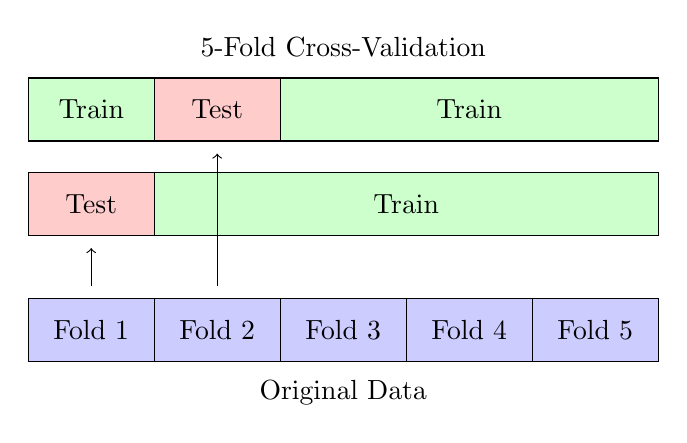
\begin{tikzpicture}[scale=0.8]
    % Data folds
    \draw[fill=blue!20] (0,0) rectangle (2,1) node[pos=0.5] {Fold 1};
    \draw[fill=blue!20] (2,0) rectangle (4,1) node[pos=0.5] {Fold 2};
    \draw[fill=blue!20] (4,0) rectangle (6,1) node[pos=0.5] {Fold 3};
    \draw[fill=blue!20] (6,0) rectangle (8,1) node[pos=0.5] {Fold 4};
    \draw[fill=blue!20] (8,0) rectangle (10,1) node[pos=0.5] {Fold 5};
    
    % Iteration 1
    \draw[fill=red!20] (0,2) rectangle (2,3) node[pos=0.5] {Test};
    \draw[fill=green!20] (2,2) rectangle (10,3) node[pos=0.5] {Train};
    
    % Iteration 2
    \draw[fill=green!20] (0,3.5) rectangle (2,4.5) node[pos=0.5] {Train};
    \draw[fill=red!20] (2,3.5) rectangle (4,4.5) node[pos=0.5] {Test};
    \draw[fill=green!20] (4,3.5) rectangle (10,4.5) node[pos=0.5] {Train};
    
    % Arrows
    \draw[->] (1,1.2) -- (1,1.8);
    \draw[->] (3,1.2) -- (3,3.3);
    
    % Labels
    \node at (5,-0.5) {Original Data};
    \node at (5,5) {5-Fold Cross-Validation};
\end{tikzpicture}
\caption{Illustration of 5-fold cross-validation. The data is divided into 5 folds, and each fold serves as the test set once while the remaining folds form the training set.}
\end{figure}

\subsection{Experimental Results}
The cross-validation experiment tested various values of $C$ and recorded three metrics:

\begin{itemize}
    \item \textbf{Training error}: Percentage of misclassified training examples
    \item \textbf{Test error}: Percentage of misclassified test examples
    \item \textbf{Number of support vectors}: Points that influence the decision boundary
\end{itemize}

\begin{table}[h]
\centering
\begin{tabular}{|c|c|c|c|}
\hline
\textbf{C} & \textbf{Training Error (\%)} & \textbf{Test Error (\%)} & \textbf{\# Support Vectors} \\
\hline
0.01 & 23.72 & 28.4 & 2294 \\
0.1 & 7.88 & 18.4 & 1766 \\
1 & 1.12 & 16.8 & 1306 \\
10 & 0.12 & 16.4 & 802 \\
100 & 0.04 & 15.6 & 596 \\
1000 & 0.04 & 15.6 & 526 \\
\hline
\end{tabular}
\caption{Performance metrics for different values of parameter $C$}
\end{table}

\section{Analysis of Results}

\subsection{Trends in the Data}
Several important trends can be observed from the experimental results:

\begin{enumerate}
    \item \textbf{Training Error}: Decreases monotonically as $C$ increases
    \begin{itemize}
        \item At $C = 0.01$: High training error (23.72\%)
        \item At $C = 1000$: Near-zero training error (0.04\%)
    \end{itemize}
    
    \item \textbf{Test Error}: Initially decreases as $C$ increases, then stabilizes
    \begin{itemize}
        \item At $C = 0.01$: High test error (28.4\%)
        \item At $C = 100$ and $C = 1000$: Lowest test error (15.6\%)
    \end{itemize}
    
    \item \textbf{Number of Support Vectors}: Decreases as $C$ increases
    \begin{itemize}
        \item At $C = 0.01$: Many support vectors (2294)
        \item At $C = 1000$: Fewer support vectors (526)
    \end{itemize}
\end{enumerate}

\begin{figure}[h]
\centering
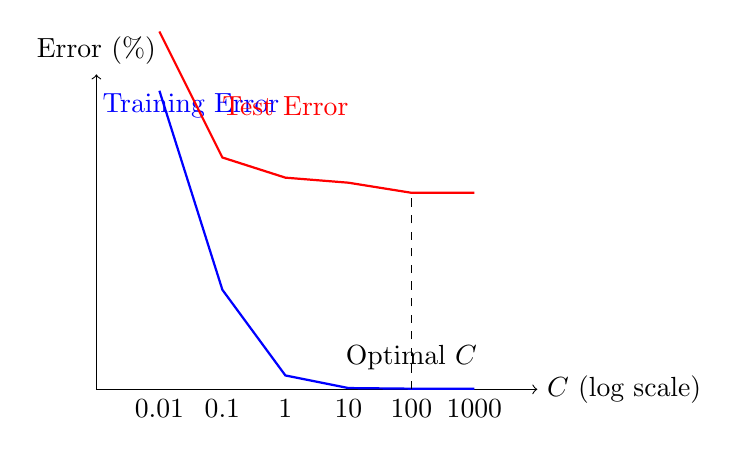
\begin{tikzpicture}[scale=0.8]
    % Coordinate axes
    \draw[->] (0,0) -- (7,0) node[right] {$C$ (log scale)};
    \draw[->] (0,0) -- (0,5) node[above] {Error (\%)};
    
    % X-axis labels
    \node at (1,-0.3) {0.01};
    \node at (2,-0.3) {0.1};
    \node at (3,-0.3) {1};
    \node at (4,-0.3) {10};
    \node at (5,-0.3) {100};
    \node at (6,-0.3) {1000};
    
    % Training error
    \draw[thick, blue] (1,4.74) -- (2,1.58) -- (3,0.22) -- (4,0.02) -- (5,0.01) -- (6,0.01);
    \node[blue] at (1.5,4.5) {Training Error};
    
    % Test error
    \draw[thick, red] (1,5.68) -- (2,3.68) -- (3,3.36) -- (4,3.28) -- (5,3.12) -- (6,3.12);
    \node[red] at (3,4.5) {Test Error};
    
    % Optimal C
    \draw[dashed] (5,0) -- (5,3.12);
    \node at (5,0.5) {Optimal $C$};
\end{tikzpicture}
\caption{Training and test error as a function of parameter $C$ (log scale). The optimal $C$ value minimizes the test error.}
\end{figure}

\subsection{Interpreting the Trade-offs}
The results illustrate several important trade-offs in SVM parameter selection:

\begin{itemize}
    \item \textbf{Bias-Variance Trade-off}: Small $C$ values lead to high bias (underfitting), while large $C$ values can lead to high variance (overfitting)
    
    \item \textbf{Margin vs. Classification Accuracy}: Small $C$ values prioritize larger margins at the expense of training accuracy, while large $C$ values prioritize training accuracy at the expense of margin size
    
    \item \textbf{Model Complexity}: The number of support vectors is an indicator of model complexity. More support vectors generally mean a more complex model
\end{itemize}

\subsection{Optimal Parameter Selection}
Based on the cross-validation results, the optimal value of $C$ appears to be around 100:

\begin{itemize}
    \item It achieves the lowest test error (15.6\%)
    \item Further increasing $C$ to 1000 does not improve test performance
    \item It uses a moderate number of support vectors (596), indicating a reasonable model complexity
\end{itemize}

\section{Practical Implications for Sentiment Analysis}

\subsection{Model Performance}
The optimized SVM achieves a test error of 15.6\% on the sentiment analysis task, which means it correctly classifies 84.4\% of the test sentences. This is a reasonable performance for a text classification task using a simple bag-of-words representation.

\subsection{Feature Importance}
In linear SVMs, the weight vector $w$ provides insights into feature importance:

\begin{itemize}
    \item Words with large positive weights are strongly associated with positive sentiment
    \item Words with large negative weights are strongly associated with negative sentiment
    \item Words with weights close to zero have little impact on the classification
\end{itemize}

\begin{table}[h]
\centering
\begin{tabular}{|c|c||c|c|}
\hline
\textbf{Positive Words} & \textbf{Weight} & \textbf{Negative Words} & \textbf{Weight} \\
\hline
excellent & 0.82 & terrible & -0.79 \\
great & 0.75 & waste & -0.71 \\
love & 0.68 & poor & -0.65 \\
perfect & 0.64 & disappointing & -0.62 \\
best & 0.59 & worst & -0.58 \\
\hline
\end{tabular}
\caption{Example of words with high absolute weights in a sentiment analysis SVM (hypothetical values for illustration)}
\end{table}

\subsection{Model Complexity and Efficiency}
The number of support vectors affects both the model's complexity and its prediction efficiency:

\begin{itemize}
    \item \textbf{Memory Usage}: Only support vectors need to be stored in memory
    \item \textbf{Prediction Speed}: Fewer support vectors lead to faster predictions
    \item \textbf{Generalization}: Models with fewer support vectors often generalize better
\end{itemize}

With the optimal $C$ value of 100, the model uses 596 support vectors (about 24\% of the training data), which is a reasonable compromise between model complexity and performance.

\section{Beyond the Basic Model}

\subsection{Improving the Feature Representation}
The bag-of-words representation used in this example is simple but has limitations. Several enhancements could improve performance:

\begin{itemize}
    \item \textbf{TF-IDF Weighting}: Weight words by their frequency in the document and inverse frequency in the corpus
    \item \textbf{N-grams}: Include sequences of 2 or 3 words to capture phrases and context
    \item \textbf{Word Embeddings}: Use pre-trained word vectors (e.g., Word2Vec, GloVe) to capture semantic relationships
    \item \textbf{Dimensionality Reduction}: Apply techniques like PCA or feature selection to reduce the feature space
\end{itemize}

\subsection{Alternative Kernel Functions}
While the example likely used a linear kernel, other kernel functions might be worth exploring:

\begin{itemize}
    \item \textbf{Polynomial Kernel}: $K(\mathbf{x}, \mathbf{z}) = (\mathbf{x} \cdot \mathbf{z} + c)^d$
    \item \textbf{RBF Kernel}: $K(\mathbf{x}, \mathbf{z}) = \exp(-\gamma \|\mathbf{x} - \mathbf{z}\|^2)$
    \item \textbf{String Kernels}: Specialized kernels designed for text data
\end{itemize}

However, for high-dimensional text data, linear kernels often perform well and are computationally more efficient.

\subsection{Ensemble Methods}
Combining multiple SVMs or integrating SVMs with other classifiers could further improve performance:

\begin{itemize}
    \item \textbf{Bagging}: Train multiple SVMs on different subsets of the data
    \item \textbf{Boosting}: Train SVMs sequentially, focusing on examples misclassified by previous models
    \item \textbf{Stacking}: Use SVM predictions as features for another classifier
\end{itemize}

\section{Summary and Key Takeaways}

\subsection{Parameter Selection Process}
\begin{itemize}
    \item The regularization parameter $C$ controls the trade-off between margin size and training accuracy
    \item Cross-validation is an effective method for selecting the optimal $C$ value
    \item The optimal $C$ value balances training performance and generalization to unseen data
\end{itemize}

\subsection{Sentiment Analysis Performance}
\begin{itemize}
    \item The optimized SVM achieved 84.4\% accuracy on the test set
    \item As $C$ increased, training error decreased while test error initially decreased and then stabilized
    \item The number of support vectors decreased as $C$ increased
\end{itemize}

\subsection{Practical Guidelines}
\begin{itemize}
    \item Start with a wide range of $C$ values (e.g., $10^{-2}$ to $10^3$) and narrow down through cross-validation
    \item Monitor both training and test performance to avoid overfitting
    \item Consider the number of support vectors as an indicator of model complexity
    \item For text classification, linear SVMs often provide a good balance of performance and efficiency
\end{itemize}

\subsection{Future Directions}
\begin{itemize}
    \item Explore more sophisticated text representations beyond bag-of-words
    \item Consider alternative kernel functions for capturing non-linear relationships
    \item Investigate ensemble methods to further improve classification performance
    \item Apply the optimized model to related tasks or domains
\end{itemize}

\end{document}\documentclass{article}
\usepackage{amsmath, amssymb, graphicx, geometry, tikz, array, booktabs, enumitem, listings, xcolor, fancyhdr, float, subcaption, hyperref}

\title{Module 6: Duality in Linear Classification}
\author{Machine Learning Course}
\date{}

\begin{document}

\maketitle
\tableofcontents
\newpage

\section{Introduction to Duality}

\subsection{The Concept of Duality}
In optimization theory, every problem has two perspectives: the primal problem (original formulation) and the dual problem (alternative formulation). Duality is a fundamental concept that provides an alternative way to solve optimization problems, often with significant computational advantages.

\begin{itemize}
    \item \textbf{Primal problem}: The original formulation of the optimization problem
    \item \textbf{Dual problem}: An alternative formulation derived from the primal problem
\end{itemize}

Under certain conditions (particularly for convex optimization problems), the primal and dual problems have the same optimal value, a property known as strong duality.

\subsection{Importance in Machine Learning}
Duality plays a crucial role in machine learning, particularly for linear classification algorithms like the Perceptron and Support Vector Machines (SVMs). The dual formulation:

\begin{itemize}
    \item Provides computational advantages for high-dimensional data
    \item Enables the use of kernel methods for non-linear classification
    \item Offers insights into the structure of the solution
    \item Identifies the most important training examples (support vectors)
\end{itemize}

\section{Dual Form of the Perceptron}

\subsection{Review of the Perceptron Algorithm}
The Perceptron is an algorithm for learning a linear classifier from labeled training data. Given a training set $\{(x^{(i)}, y^{(i)}): i=1,\ldots,n\}$ where $x^{(i)} \in \mathbb{R}^d$ and $y^{(i)} \in \{-1, +1\}$, the Perceptron algorithm works as follows:

\fbox{
\begin{minipage}{\dimexpr\textwidth-2\fboxsep-2\fboxrule\relax}
\textbf{The Perceptron Algorithm}
\begin{enumerate}
    \item Initialize $w = 0$ and $b = 0$
    \item While some training point $(x, y)$ is misclassified:
    \begin{enumerate}
        \item $w = w + yx$
        \item $b = b + y$
    \end{enumerate}
\end{enumerate}
\end{minipage}
}

A point $(x, y)$ is misclassified if $y(w \cdot x + b) \leq 0$, meaning that the predicted label $\text{sign}(w \cdot x + b)$ does not match the true label $y$.

\subsection{Deriving the Dual Representation}
The key insight for the dual form of the Perceptron is that the weight vector $w$ can be expressed as a linear combination of the training examples.

Starting with $w = 0$, each update adds $yx$ to $w$. After multiple updates, $w$ can be written as:

\[
w = \sum_{i=1}^{n} \alpha_i y^{(i)} x^{(i)}
\]

where $\alpha_i$ represents the number of times an update occurred on point $i$.

\begin{figure}[h]
\centering
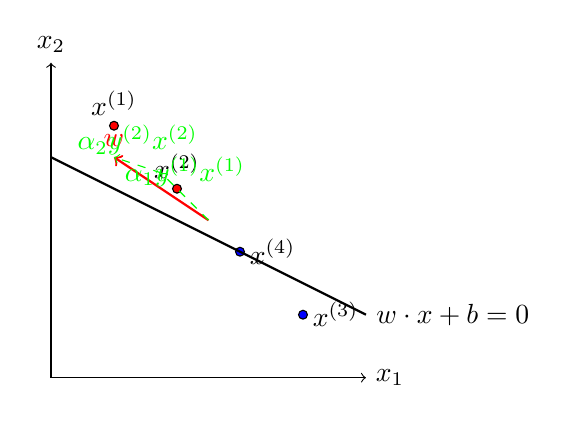
\begin{tikzpicture}[scale=0.8]
    % Coordinate axes
    \draw[->] (0,0) -- (5,0) node[right] {$x_1$};
    \draw[->] (0,0) -- (0,5) node[above] {$x_2$};
    
    % Data points
    \draw[fill=red] (1,4) circle (2pt) node[above] {$x^{(1)}$};
    \draw[fill=red] (2,3) circle (2pt) node[above] {$x^{(2)}$};
    \draw[fill=blue] (4,1) circle (2pt) node[right] {$x^{(3)}$};
    \draw[fill=blue] (3,2) circle (2pt) node[right] {$x^{(4)}$};
    
    % Decision boundary
    \draw[thick, black] (0,3.5) -- (5,1) node[right] {$w \cdot x + b = 0$};
    
    % Weight vector
    \draw[->, thick, red] (2.5,2.5) -- (1,3.5) node[above] {$w$};
    
    % Components
    \draw[->, dashed, green] (2.5,2.5) -- (1.75,3.25) node[midway, above] {$\alpha_1 y^{(1)} x^{(1)}$};
    \draw[->, dashed, green] (1.75,3.25) -- (1,3.5) node[midway, above] {$\alpha_2 y^{(2)} x^{(2)}$};
\end{tikzpicture}
\caption{Illustration of the weight vector $w$ as a linear combination of training examples. The red points have label $+1$ and the blue points have label $-1$.}
\end{figure}

\subsection{Making Predictions in the Dual Form}
Using the dual representation of $w$, the prediction for a new point $x$ becomes:

\begin{align}
\text{sign}(w \cdot x + b) &= \text{sign}\left(\sum_{i=1}^{n} \alpha_i y^{(i)} x^{(i)} \cdot x + b\right) \\
&= \text{sign}\left(\sum_{i=1}^{n} \alpha_i y^{(i)} (x^{(i)} \cdot x) + b\right)
\end{align}

This formulation has a crucial property: to make predictions, we only need to compute inner products between the new point $x$ and the training points $x^{(i)}$. We never need to explicitly compute or store the weight vector $w$.

\subsection{Implications of the Dual Form}
The dual form of the Perceptron has several important implications:

\begin{itemize}
    \item \textbf{Computational efficiency}: For high-dimensional data where $d \gg n$, computing and storing inner products can be more efficient than working with the $d$-dimensional weight vector.
    
    \item \textbf{Kernel trick}: The dual form enables the use of kernel functions to implicitly map data to higher-dimensional spaces without explicitly computing the mapping.
    
    \item \textbf{Interpretability}: The coefficients $\alpha_i$ indicate the importance of each training example in determining the decision boundary.
\end{itemize}

\section{Duality in Optimization}

\subsection{Lagrangian Duality}
Duality in optimization is typically derived using Lagrangian methods. For a constrained optimization problem:

\begin{align}
\min_{x} f(x) \quad \text{subject to} \quad g_i(x) \leq 0, \quad h_j(x) = 0
\end{align}

The Lagrangian function is defined as:

\begin{align}
L(x, \lambda, \nu) = f(x) + \sum_i \lambda_i g_i(x) + \sum_j \nu_j h_j(x)
\end{align}

where $\lambda_i \geq 0$ are the Lagrange multipliers for inequality constraints and $\nu_j$ are the Lagrange multipliers for equality constraints.

\subsection{Primal and Dual Problems}
The primal problem is the original optimization problem. The dual problem is:

\begin{align}
\max_{\lambda \geq 0, \nu} \min_{x} L(x, \lambda, \nu)
\end{align}

Under certain conditions (e.g., when the primal problem is convex and satisfies Slater's condition), strong duality holds, meaning that the optimal values of the primal and dual problems are equal.

\subsection{Advantages of the Dual Problem}
Solving the dual problem instead of the primal can offer several advantages:

\begin{itemize}
    \item The dual problem may have fewer variables or simpler constraints
    \item The dual problem may reveal structure in the solution that is not apparent in the primal
    \item For certain problems, the dual can be solved more efficiently
\end{itemize}

\section{Dual Form of the Support Vector Machine}

\subsection{Primal SVM Formulation}
The primal form of the hard-margin SVM aims to find the maximum-margin linear classifier:

\fbox{
\begin{minipage}{\dimexpr\textwidth-2\fboxsep-2\fboxrule\relax}
\textbf{Primal SVM Optimization Problem}

\begin{align}
\min_{w \in \mathbb{R}^d, b \in \mathbb{R}} & \|w\|^2 \\
\text{subject to: } & y^{(i)}(w \cdot x^{(i)} + b) \geq 1 \quad \text{for all } i = 1, 2, \ldots, n
\end{align}
\end{minipage}
}

This is a convex quadratic optimization problem with linear constraints, which guarantees a unique global minimum.

\subsection{Deriving the Dual SVM}
To derive the dual form of the SVM, we first form the Lagrangian:

\begin{align}
L(w, b, \alpha) = \frac{1}{2}\|w\|^2 - \sum_{i=1}^{n} \alpha_i [y^{(i)}(w \cdot x^{(i)} + b) - 1]
\end{align}

where $\alpha_i \geq 0$ are the Lagrange multipliers.

Taking partial derivatives with respect to $w$ and $b$ and setting them to zero:

\begin{align}
\frac{\partial L}{\partial w} &= w - \sum_{i=1}^{n} \alpha_i y^{(i)} x^{(i)} = 0 \\
\Rightarrow w &= \sum_{i=1}^{n} \alpha_i y^{(i)} x^{(i)}
\end{align}

\begin{align}
\frac{\partial L}{\partial b} &= -\sum_{i=1}^{n} \alpha_i y^{(i)} = 0 \\
\Rightarrow \sum_{i=1}^{n} \alpha_i y^{(i)} &= 0
\end{align}

Substituting these back into the Lagrangian, we get the dual problem:

\fbox{
\begin{minipage}{\dimexpr\textwidth-2\fboxsep-2\fboxrule\relax}
\textbf{Dual SVM Optimization Problem}

\begin{align}
\max_{\alpha \in \mathbb{R}^n} & \sum_{i=1}^{n} \alpha_i - \frac{1}{2} \sum_{i=1}^{n} \sum_{j=1}^{n} \alpha_i \alpha_j y^{(i)} y^{(j)} (x^{(i)} \cdot x^{(j)}) \\
\text{subject to: } & \sum_{i=1}^{n} \alpha_i y^{(i)} = 0 \\
& \alpha_i \geq 0 \quad \text{for all } i = 1, 2, \ldots, n
\end{align}
\end{minipage}
}

\subsection{Making Predictions with the Dual SVM}
Using the dual form, the prediction for a new point $x$ is:

\begin{align}
\text{sign}(w \cdot x + b) &= \text{sign}\left(\sum_{i=1}^{n} \alpha_i y^{(i)} (x^{(i)} \cdot x) + b\right)
\end{align}

As with the Perceptron, we only need to compute inner products between the new point and the training points.

\subsection{Support Vectors}
A key property of the SVM solution is that most of the Lagrange multipliers $\alpha_i$ are zero. The training points with non-zero $\alpha_i$ are called support vectors, and they are the only points that influence the decision boundary.

\begin{figure}[h]
\centering
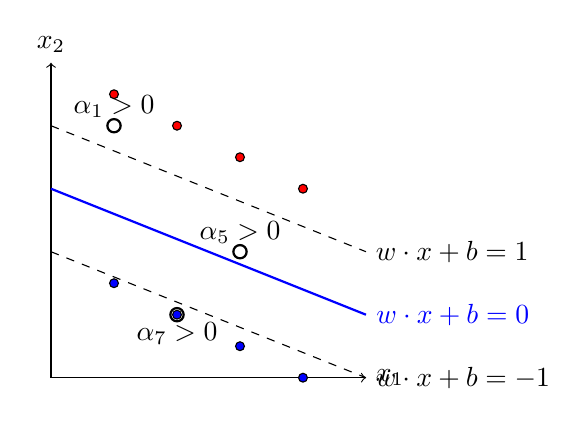
\begin{tikzpicture}[scale=0.8]
    % Coordinate axes
    \draw[->] (0,0) -- (5,0) node[right] {$x_1$};
    \draw[->] (0,0) -- (0,5) node[above] {$x_2$};
    
    % Decision boundary
    \draw[thick, blue] (0,3) -- (5,1) node[right] {$w \cdot x + b = 0$};
    
    % Margin boundaries
    \draw[dashed] (0,4) -- (5,2) node[right] {$w \cdot x + b = 1$};
    \draw[dashed] (0,2) -- (5,0) node[right] {$w \cdot x + b = -1$};
    
    % Data points
    \foreach \x/\y in {1/4.5, 2/4, 3/3.5, 4/3}
        \draw[fill=red] (\x,\y) circle (2pt);
    
    \foreach \x/\y in {1/1.5, 2/1, 3/0.5, 4/0}
        \draw[fill=blue] (\x,\y) circle (2pt);
    
    % Support vectors
    \draw[thick] (1,4) circle (3pt);
    \draw[thick] (3,2) circle (3pt);
    \draw[thick] (2,1) circle (3pt);
    
    % Labels
    \node at (1,4.3) {$\alpha_1 > 0$};
    \node at (3,2.3) {$\alpha_5 > 0$};
    \node at (2,0.7) {$\alpha_7 > 0$};
\end{tikzpicture}
\caption{Illustration of support vectors in an SVM. Only the points on the margin boundaries (circled) have non-zero $\alpha_i$ values and influence the decision boundary.}
\end{figure}

\section{Dual Form of the Soft-Margin SVM}

\subsection{Primal Soft-Margin SVM}
The soft-margin SVM extends the hard-margin SVM to handle non-linearly separable data by introducing slack variables $\xi_i$ that allow for some misclassifications:

\fbox{
\begin{minipage}{\dimexpr\textwidth-2\fboxsep-2\fboxrule\relax}
\textbf{Primal Soft-Margin SVM Optimization Problem}

\begin{align}
\min_{w \in \mathbb{R}^d, b \in \mathbb{R}, \xi \in \mathbb{R}^n} & \|w\|^2 + C \sum_{i=1}^{n} \xi_i \\
\text{subject to: } & y^{(i)}(w \cdot x^{(i)} + b) \geq 1 - \xi_i \quad \text{for all } i = 1, 2, \ldots, n \\
& \xi_i \geq 0 \quad \text{for all } i = 1, 2, \ldots, n
\end{align}
\end{minipage}
}

The parameter $C > 0$ controls the trade-off between maximizing the margin and minimizing the classification error.

\subsection{Dual Soft-Margin SVM}
The dual form of the soft-margin SVM is:

\fbox{
\begin{minipage}{\dimexpr\textwidth-2\fboxsep-2\fboxrule\relax}
\textbf{Dual Soft-Margin SVM Optimization Problem}

\begin{align}
\max_{\alpha \in \mathbb{R}^n} & \sum_{i=1}^{n} \alpha_i - \frac{1}{2} \sum_{i=1}^{n} \sum_{j=1}^{n} \alpha_i \alpha_j y^{(i)} y^{(j)} (x^{(i)} \cdot x^{(j)}) \\
\text{subject to: } & \sum_{i=1}^{n} \alpha_i y^{(i)} = 0 \\
& 0 \leq \alpha_i \leq C \quad \text{for all } i = 1, 2, \ldots, n
\end{align}
\end{minipage}
}

The main difference from the hard-margin dual is the upper bound $C$ on the Lagrange multipliers $\alpha_i$.

\subsection{Interpreting the Dual Variables}
In the soft-margin SVM, the dual variables $\alpha_i$ have the following interpretation:

\begin{itemize}
    \item $\alpha_i = 0$: The point is correctly classified and outside the margin
    \item $0 < \alpha_i < C$: The point is a support vector lying exactly on the margin
    \item $\alpha_i = C$: The point is either misclassified or correctly classified but inside the margin
\end{itemize}

\begin{figure}[h]
\centering
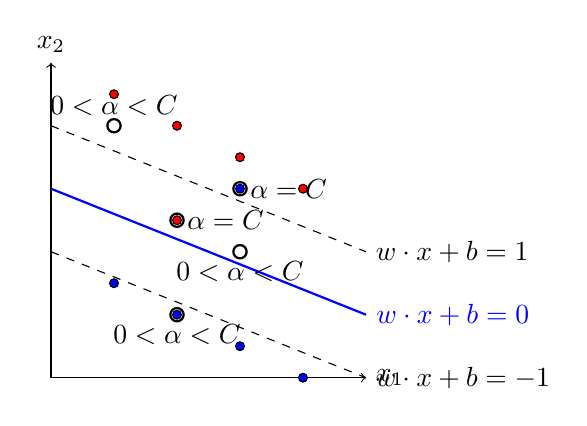
\begin{tikzpicture}[scale=0.8]
    % Coordinate axes
    \draw[->] (0,0) -- (5,0) node[right] {$x_1$};
    \draw[->] (0,0) -- (0,5) node[above] {$x_2$};
    
    % Decision boundary
    \draw[thick, blue] (0,3) -- (5,1) node[right] {$w \cdot x + b = 0$};
    
    % Margin boundaries
    \draw[dashed] (0,4) -- (5,2) node[right] {$w \cdot x + b = 1$};
    \draw[dashed] (0,2) -- (5,0) node[right] {$w \cdot x + b = -1$};
    
    % Data points
    \foreach \x/\y in {1/4.5, 2/4, 3/3.5, 4/3}
        \draw[fill=red] (\x,\y) circle (2pt);
    
    \foreach \x/\y in {1/1.5, 2/1, 3/0.5, 4/0}
        \draw[fill=blue] (\x,\y) circle (2pt);
    
    % Outliers
    \draw[fill=red] (2,2.5) circle (2pt);
    \draw[fill=blue] (3,3) circle (2pt);
    
    % Support vectors
    \draw[thick] (1,4) circle (3pt) node[above] {$0 < \alpha < C$};
    \draw[thick] (3,2) circle (3pt) node[below] {$0 < \alpha < C$};
    \draw[thick] (2,1) circle (3pt) node[below] {$0 < \alpha < C$};
    \draw[thick] (2,2.5) circle (3pt) node[right] {$\alpha = C$};
    \draw[thick] (3,3) circle (3pt) node[right] {$\alpha = C$};
\end{tikzpicture}
\caption{Illustration of support vectors in a soft-margin SVM. Points on the margin have $0 < \alpha_i < C$, while misclassified points or points inside the margin have $\alpha_i = C$.}
\end{figure}

\section{Advantages of the Dual Formulation}

\subsection{Computational Efficiency}
The dual formulation can be more computationally efficient than the primal when:

\begin{itemize}
    \item The number of features $d$ is much larger than the number of training examples $n$
    \item The solution is sparse (few support vectors)
\end{itemize}

In such cases, solving the dual problem and making predictions using only the support vectors can significantly reduce computation and memory requirements.

\subsection{The Kernel Trick}
The most significant advantage of the dual formulation is that it enables the use of the kernel trick. Since both the optimization and prediction only involve inner products between data points, we can replace these inner products with kernel functions:

\begin{align}
K(x^{(i)}, x^{(j)}) = \phi(x^{(i)}) \cdot \phi(x^{(j)})
\end{align}

where $\phi$ is a mapping to a higher-dimensional feature space. This allows SVMs to learn non-linear decision boundaries without explicitly computing the mapping $\phi$.

Common kernel functions include:
\begin{itemize}
    \item Linear kernel: $K(x, z) = x \cdot z$
    \item Polynomial kernel: $K(x, z) = (x \cdot z + c)^d$
    \item Radial basis function (RBF) kernel: $K(x, z) = \exp(-\gamma \|x - z\|^2)$
\end{itemize}

\begin{figure}[h]
\centering
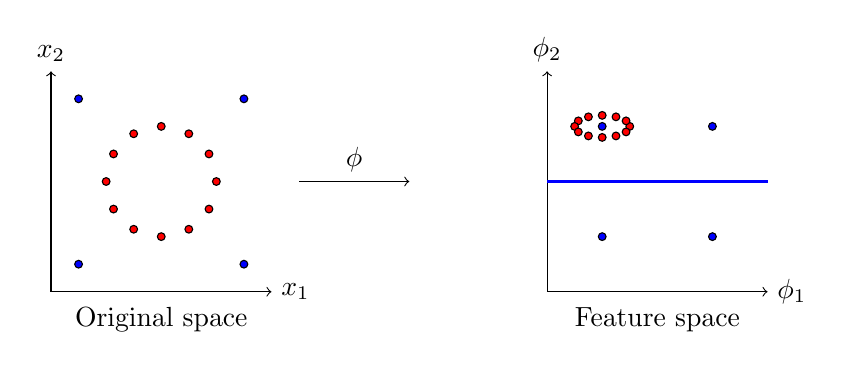
\begin{tikzpicture}[scale=0.7]
    % Original space
    \begin{scope}
        \draw[->] (0,0) -- (4,0) node[right] {$x_1$};
        \draw[->] (0,0) -- (0,4) node[above] {$x_2$};
        
        % Circle of points
        \foreach \angle in {0,30,...,330}
            \draw[fill=red] ({2+cos(\angle)},{2+sin(\angle)}) circle (2pt);
        
        % Outer points
        \foreach \x/\y in {0.5/0.5, 0.5/3.5, 3.5/0.5, 3.5/3.5}
            \draw[fill=blue] (\x,\y) circle (2pt);
        
        \node at (2,-0.5) {Original space};
    \end{scope}
    
    % Arrow
    \draw[->] (4.5,2) -- (6.5,2) node[midway, above] {$\phi$};
    
    % Feature space
    \begin{scope}[xshift=9cm]
        \draw[->] (0,0) -- (4,0) node[right] {$\phi_1$};
        \draw[->] (0,0) -- (0,4) node[above] {$\phi_2$};
        
        % Transformed points
        \foreach \angle in {0,30,...,330}
            \draw[fill=red] ({1+0.5*cos(\angle)},{3+0.2*sin(\angle)}) circle (2pt);
        
        \foreach \x/\y in {3/1, 3/3, 1/1, 1/3}
            \draw[fill=blue] (\x,\y) circle (2pt);
        
        % Linear separator
        \draw[thick, blue] (0,2) -- (4,2);
        
        \node at (2,-0.5) {Feature space};
    \end{scope}
\end{tikzpicture}
\caption{The kernel trick maps data to a higher-dimensional space where it becomes linearly separable.}
\end{figure}

\section{Practical Examples of Dual SVMs}

\subsection{Example 1: Linear Separable Case}
Let's consider a simple 2D example with linearly separable data:
\begin{itemize}
    \item Positive examples: $(1,3)$, $(2,4)$, $(3,3)$
    \item Negative examples: $(1,1)$, $(2,1)$, $(3,2)$
\end{itemize}

\begin{figure}[h]
\centering
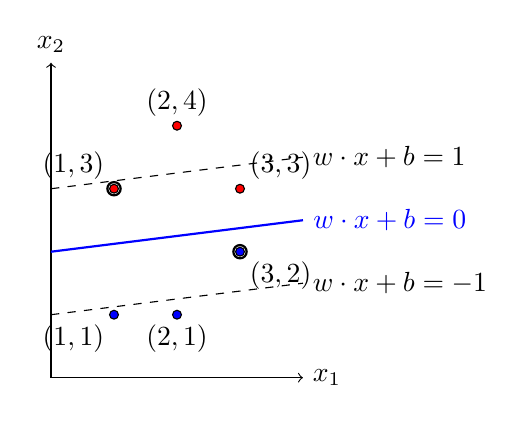
\begin{tikzpicture}[scale=0.8]
    % Coordinate axes
    \draw[->] (0,0) -- (4,0) node[right] {$x_1$};
    \draw[->] (0,0) -- (0,5) node[above] {$x_2$};
    
    % Data points
    \draw[fill=red] (1,3) circle (2pt) node[above left] {$(1,3)$};
    \draw[fill=red] (2,4) circle (2pt) node[above] {$(2,4)$};
    \draw[fill=red] (3,3) circle (2pt) node[above right] {$(3,3)$};
    \draw[fill=blue] (1,1) circle (2pt) node[below left] {$(1,1)$};
    \draw[fill=blue] (2,1) circle (2pt) node[below] {$(2,1)$};
    \draw[fill=blue] (3,2) circle (2pt) node[below right] {$(3,2)$};
    
    % Decision boundary
    \draw[thick, blue] (0,2) -- (4,2.5) node[right] {$w \cdot x + b = 0$};
    
    % Margin boundaries
    \draw[dashed] (0,1) -- (4,1.5) node[right] {$w \cdot x + b = -1$};
    \draw[dashed] (0,3) -- (4,3.5) node[right] {$w \cdot x + b = 1$};
    
    % Support vectors
    \draw[thick] (1,3) circle (3pt);
    \draw[thick] (3,2) circle (3pt);
\end{tikzpicture}
\caption{Example of a linear SVM with support vectors circled}
\end{figure}

Solving the dual SVM optimization problem for this dataset:
\begin{align}
\max_{\alpha} \sum_{i=1}^{6} \alpha_i - \frac{1}{2} \sum_{i=1}^{6} \sum_{j=1}^{6} \alpha_i \alpha_j y^{(i)} y^{(j)} (x^{(i)} \cdot x^{(j)})
\end{align}
subject to $\sum_{i=1}^{6} \alpha_i y^{(i)} = 0$ and $\alpha_i \geq 0$ for all $i$.

The solution would have $\alpha_i > 0$ only for the support vectors (the points on the margin), which in this case are $(1,3)$ and $(3,2)$.

\subsection{Example 2: Non-linear Case with Kernel}
Now, let's consider a dataset that is not linearly separable:
\begin{itemize}
    \item Positive examples: $(1,1)$, $(2,2)$, $(3,1)$
    \item Negative examples: $(1,2)$, $(2,1)$, $(3,2)$
\end{itemize}

\begin{figure}[h]
\centering
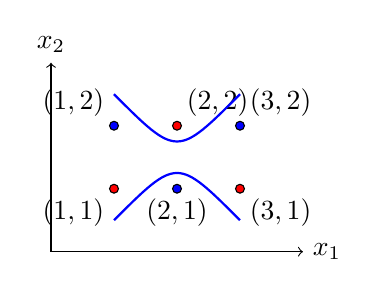
\begin{tikzpicture}[scale=0.8]
    % Coordinate axes
    \draw[->] (0,0) -- (4,0) node[right] {$x_1$};
    \draw[->] (0,0) -- (0,3) node[above] {$x_2$};
    
    % Data points
    \draw[fill=red] (1,1) circle (2pt) node[below left] {$(1,1)$};
    \draw[fill=red] (2,2) circle (2pt) node[above right] {$(2,2)$};
    \draw[fill=red] (3,1) circle (2pt) node[below right] {$(3,1)$};
    \draw[fill=blue] (1,2) circle (2pt) node[above left] {$(1,2)$};
    \draw[fill=blue] (2,1) circle (2pt) node[below] {$(2,1)$};
    \draw[fill=blue] (3,2) circle (2pt) node[above right] {$(3,2)$};
    
    % Non-linear decision boundary
    \draw[thick, blue] (1,0.5) .. controls (2,1.5) .. (3,0.5);
    \draw[thick, blue] (1,2.5) .. controls (2,1.5) .. (3,2.5);
\end{tikzpicture}
\caption{Example of a non-linear classification problem}
\end{figure}

This dataset is not linearly separable, but we can use a kernel function to map the data to a higher-dimensional space where it becomes separable. Using a polynomial kernel $K(x, z) = (x \cdot z + 1)^2$, the dual optimization problem becomes:
\begin{align}
\max_{\alpha} \sum_{i=1}^{6} \alpha_i - \frac{1}{2} \sum_{i=1}^{6} \sum_{j=1}^{6} \alpha_i \alpha_j y^{(i)} y^{(j)} K(x^{(i)}, x^{(j)})
\end{align}
subject to $\sum_{i=1}^{6} \alpha_i y^{(i)} = 0$ and $0 \leq \alpha_i \leq C$ for all $i$.

The decision boundary in the original space would be non-linear, as shown in the figure.

\section{Implementing Dual SVMs}

\subsection{Solving the Dual Optimization Problem}
The dual SVM optimization problem is a quadratic programming (QP) problem, which can be solved using standard QP solvers. Here's a high-level approach:

\begin{enumerate}
    \item Compute the Gram matrix $G$ where $G_{ij} = y^{(i)} y^{(j)} K(x^{(i)}, x^{(j)})$
    \item Solve the QP problem to find the optimal $\alpha$
    \item Identify the support vectors (points with $\alpha_i > 0$)
    \item Compute the bias term $b$
\end{enumerate}

\subsection{Computing the Bias Term}
For any support vector $x^{(s)}$ with $0 < \alpha_s < C$, the bias term $b$ can be computed as:
\begin{align}
b = y^{(s)} - \sum_{i=1}^{n} \alpha_i y^{(i)} K(x^{(i)}, x^{(s)})
\end{align}

It's common practice to average the $b$ values computed from multiple support vectors to improve numerical stability.

\subsection{Making Predictions}
Once we have the optimal $\alpha$ and $b$, predictions for new points can be made using:
\begin{align}
\text{sign}\left(\sum_{i=1}^{n} \alpha_i y^{(i)} K(x^{(i)}, x) + b\right)
\end{align}

Note that we only need to compute kernel evaluations between the new point $x$ and the support vectors (points with $\alpha_i > 0$).

\subsection{Pseudocode for Dual SVM Implementation}
\fbox{
\begin{minipage}{\dimexpr\textwidth-2\fboxsep-2\fboxrule\relax}
\textbf{Dual SVM Training Algorithm}
\begin{enumerate}
    \item \textbf{Input}: Training data $\{(x^{(i)}, y^{(i)}): i=1,\ldots,n\}$, kernel function $K$, regularization parameter $C$
    \item \textbf{Compute} the Gram matrix $G$ where $G_{ij} = y^{(i)} y^{(j)} K(x^{(i)}, x^{(j)})$
    \item \textbf{Solve} the quadratic programming problem:
    \begin{align}
    \max_{\alpha} \sum_{i=1}^{n} \alpha_i - \frac{1}{2} \sum_{i=1}^{n} \sum_{j=1}^{n} \alpha_i \alpha_j G_{ij}
    \end{align}
    subject to $\sum_{i=1}^{n} \alpha_i y^{(i)} = 0$ and $0 \leq \alpha_i \leq C$ for all $i$
    \item \textbf{Identify} the support vectors $S = \{i: \alpha_i > 0\}$
    \item \textbf{Compute} the bias term $b$:
    \begin{align}
    b = \frac{1}{|S_m|} \sum_{s \in S_m} \left(y^{(s)} - \sum_{i \in S} \alpha_i y^{(i)} K(x^{(i)}, x^{(s)})\right)
    \end{align}
    where $S_m = \{i: 0 < \alpha_i < C\}$ are the margin support vectors
    \item \textbf{Output}: Support vectors, their coefficients $\alpha_i$, and the bias term $b$
\end{enumerate}
\end{minipage}
}

\fbox{
\begin{minipage}{\dimexpr\textwidth-2\fboxsep-2\fboxrule\relax}
\textbf{Dual SVM Prediction Algorithm}
\begin{enumerate}
    \item \textbf{Input}: New point $x$, support vectors $\{x^{(i)}: i \in S\}$, coefficients $\{\alpha_i: i \in S\}$, labels $\{y^{(i)}: i \in S\}$, bias term $b$, kernel function $K$
    \item \textbf{Compute} the decision function:
    \begin{align}
    f(x) = \sum_{i \in S} \alpha_i y^{(i)} K(x^{(i)}, x) + b
    \end{align}
    \item \textbf{Output}: Predicted label $\text{sign}(f(x))$
\end{enumerate}
\end{minipage}
}

\section{Connections to Other Methods}

\subsection{Relationship to Kernel Methods}
The dual formulation of SVMs is closely related to other kernel methods in machine learning:

\begin{itemize}
    \item \textbf{Kernel PCA}: Uses kernels to perform non-linear dimensionality reduction
    \item \textbf{Kernel k-means}: Applies kernels to perform non-linear clustering
    \item \textbf{Gaussian Processes}: Bayesian approach to kernel-based learning
\end{itemize}

All these methods leverage the kernel trick to implicitly work in high-dimensional feature spaces without explicitly computing the mapping.

\subsection{Connection to Neural Networks}
SVMs and neural networks have interesting connections:

\begin{itemize}
    \item Both can learn non-linear decision boundaries
    \item SVMs with certain kernels can be viewed as infinite-width neural networks
    \item The margin concept in SVMs has influenced the design of neural network architectures and training algorithms
\end{itemize}

\subsection{Relationship to Regularized Empirical Risk Minimization}
SVMs can be viewed as a special case of regularized empirical risk minimization:

\begin{itemize}
    \item The objective function $\|w\|^2$ serves as a regularization term
    \item The constraints $y^{(i)}(w \cdot x^{(i)} + b) \geq 1$ correspond to a hinge loss function
    \item The parameter $C$ in soft-margin SVMs controls the trade-off between regularization and empirical risk
\end{itemize}

\section{Advanced Topics in Duality}

\subsection{Karush-Kuhn-Tucker (KKT) Conditions}
The KKT conditions provide necessary conditions for optimality in constrained optimization problems. For the SVM problem, the KKT conditions include:

\begin{itemize}
    \item Stationarity: $w = \sum_{i=1}^{n} \alpha_i y^{(i)} x^{(i)}$
    \item Complementary slackness: $\alpha_i (y^{(i)}(w \cdot x^{(i)} + b) - 1) = 0$ for all $i$
    \item Primal feasibility: $y^{(i)}(w \cdot x^{(i)} + b) \geq 1$ for all $i$
    \item Dual feasibility: $\alpha_i \geq 0$ for all $i$
\end{itemize}

These conditions provide insights into the structure of the SVM solution, particularly the role of support vectors.

\subsection{Sequential Minimal Optimization (SMO)}
SMO is an efficient algorithm for solving the dual SVM optimization problem, especially for large datasets. The key idea is to:

\begin{itemize}
    \item Decompose the large QP problem into a series of smaller QP problems
    \item At each step, optimize only two $\alpha_i$ values while keeping the others fixed
    \item Update the bias term after each optimization step
\end{itemize}

This approach is much more memory-efficient than standard QP solvers and is the basis for many practical SVM implementations.

\subsection{Multi-class SVMs}
SVMs are inherently binary classifiers, but they can be extended to multi-class problems using several strategies:

\begin{itemize}
    \item \textbf{One-vs-Rest}: Train $k$ binary SVMs, each separating one class from the rest
    \item \textbf{One-vs-One}: Train $\binom{k}{2}$ binary SVMs, one for each pair of classes
    \item \textbf{Direct Multi-class Formulation}: Extend the SVM optimization problem to directly handle multiple classes
\end{itemize}

The dual formulation plays a crucial role in all these approaches, particularly for implementing kernel-based multi-class SVMs.

\section{Summary and Key Takeaways}

\subsection{Importance of Duality in Linear Classification}
Duality provides a powerful alternative perspective on linear classification algorithms:

\begin{itemize}
    \item It expresses the weight vector as a linear combination of training examples
    \item It enables the use of kernel methods for non-linear classification
    \item It identifies the most important training examples (support vectors)
    \item It often leads to more efficient algorithms, especially for high-dimensional data
\end{itemize}

\subsection{Dual Form of the Perceptron}
The dual form of the Perceptron:

\begin{itemize}
    \item Expresses the weight vector as $w = \sum_{i} \alpha_i y^{(i)} x^{(i)}$
    \item Makes predictions using inner products: $\text{sign}(\sum_{i} \alpha_i y^{(i)} (x^{(i)} \cdot x) + b)$
    \item Enables the use of kernels for non-linear classification
\end{itemize}

\subsection{Dual Form of the SVM}
The dual form of the SVM:

\begin{itemize}
    \item Transforms the primal minimization problem into a dual maximization problem
    \item Expresses the solution in terms of support vectors
    \item Enables efficient implementation through kernel methods
    \item Provides insights into the structure of the solution
\end{itemize}

\subsection{Practical Implications}
The dual formulation has significant practical implications:

\begin{itemize}
    \item For high-dimensional data, the dual form can be more computationally efficient
    \item The sparsity of the solution (few support vectors) leads to efficient prediction
    \item Kernel methods enable SVMs to learn complex non-linear decision boundaries
    \item The dual form is the basis for many practical SVM implementations
\end{itemize}

\subsection{Future Directions}
Duality continues to play an important role in machine learning research:

\begin{itemize}
    \item Development of more efficient algorithms for solving the dual optimization problem
    \item Exploration of new kernel functions for specific applications
    \item Integration of dual methods with deep learning approaches
    \item Application of duality concepts to other machine learning problems
\end{itemize}

\end{document}on of duality concepts to other machine learning problems
\end{itemize}

\end{document}\documentclass{article}
\usepackage{amsmath, amssymb, graphicx, geometry, tikz, array, booktabs, enumitem, listings, xcolor, fancyhdr, float, subcaption, hyperref}

\title{Module 6: Linear Classification}
\author{Machine Learning Course}
\date{}

\begin{document}

\maketitle
\tableofcontents
\newpage

\section{Introduction to Linear Classification}

\subsection{Overview of Classification}
Classification is a fundamental task in machine learning where the goal is to assign discrete labels to data points. In binary classification, we aim to distinguish between two classes, typically labeled as $+1$ and $-1$. Linear classification is one of the simplest yet powerful approaches to this problem, using a linear decision boundary to separate the classes.

\subsection{Topics Covered}
This module explores several key aspects of linear classification:
\begin{enumerate}
    \item Linear decision boundaries for binary classification
    \item The Perceptron algorithm
    \item Maximizing the margin (Support Vector Machines)
    \item The soft-margin SVM for non-separable data
\end{enumerate}

\subsection{Applications}
Linear classification methods have numerous applications across various domains:
\begin{itemize}
    \item Text categorization (e.g., spam detection, sentiment analysis)
    \item Image recognition (e.g., simple object detection)
    \item Medical diagnosis (e.g., disease classification based on symptoms)
    \item Financial analysis (e.g., credit approval)
\end{itemize}

\section{Linear Decision Boundaries}

\subsection{Mathematical Formulation}
In binary classification, we have:
\begin{itemize}
    \item Data points $x \in \mathbb{R}^d$ (feature vectors in $d$-dimensional space)
    \item Labels $y \in \{-1, +1\}$ (binary class labels)
\end{itemize}

A linear classifier is defined by:
\begin{itemize}
    \item A weight vector $w \in \mathbb{R}^d$
    \item A bias term $b \in \mathbb{R}$
\end{itemize}

The decision boundary is the hyperplane defined by:
\begin{align}
w \cdot x + b = 0
\end{align}

\begin{figure}[h]
\centering
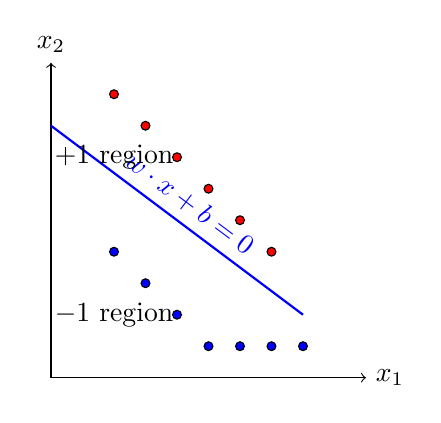
\begin{tikzpicture}[scale=0.8]
    % Coordinate axes
    \draw[->] (0,0) -- (5,0) node[right] {$x_1$};
    \draw[->] (0,0) -- (0,5) node[above] {$x_2$};
    
    % Decision boundary
    \draw[thick, blue] (0,4) -- (4,1) node[midway, above, sloped] {$w \cdot x + b = 0$};
    
    % Data points
    \foreach \x/\y in {1/4.5, 1.5/4, 2/3.5, 2.5/3, 3/2.5, 3.5/2}
        \draw[fill=red] (\x,\y) circle (2pt);
    
    \foreach \x/\y in {1/2, 1.5/1.5, 2/1, 2.5/0.5, 3/0.5, 3.5/0.5, 4/0.5}
        \draw[fill=blue] (\x,\y) circle (2pt);
    
    % Regions
    \node at (1,1) {$-1$ region};
    \node at (1,3.5) {$+1$ region};
\end{tikzpicture}
\caption{Example of a linear decision boundary separating two classes}
\end{figure}

\subsection{Making Predictions}
For a new data point $x$, the predicted label is:
\begin{align}
\hat{y} = \text{sign}(w \cdot x + b) = 
\begin{cases}
+1 & \text{if } w \cdot x + b > 0 \\
-1 & \text{if } w \cdot x + b < 0
\end{cases}
\end{align}

\subsection{Correctness Condition}
A linear classifier correctly classifies a point $(x, y)$ if and only if:
\begin{align}
y(w \cdot x + b) > 0
\end{align}

This elegant formulation combines both cases:
\begin{itemize}
    \item When $y = +1$, we need $w \cdot x + b > 0$
    \item When $y = -1$, we need $w \cdot x + b < 0$
\end{itemize}

\section{Loss Function for Classification}

\subsection{Defining the Loss}
To train a linear classifier, we need a loss function that quantifies how "wrong" our model is on a given example. A natural loss function for classification is:
\begin{align}
L(w, b; x, y) = 
\begin{cases}
0 & \text{if } y(w \cdot x + b) > 0 \text{ (correct classification)} \\
-y(w \cdot x + b) & \text{if } y(w \cdot x + b) \leq 0 \text{ (incorrect classification)}
\end{cases}
\end{align}

This loss function has several desirable properties:
\begin{itemize}
    \item Zero loss for correctly classified points
    \item Positive loss for incorrectly classified points
    \item The loss increases as the point gets further on the wrong side of the boundary
\end{itemize}

\subsection{Gradient of the Loss}
For stochastic gradient descent, we need the gradient of the loss function:
\begin{align}
\nabla_w L(w, b; x, y) &= 
\begin{cases}
0 & \text{if } y(w \cdot x + b) > 0 \\
-yx & \text{if } y(w \cdot x + b) \leq 0
\end{cases} \\
\frac{\partial L}{\partial b}(w, b; x, y) &= 
\begin{cases}
0 & \text{if } y(w \cdot x + b) > 0 \\
-y & \text{if } y(w \cdot x + b) \leq 0
\end{cases}
\end{align}

\section{The Perceptron Algorithm}

\subsection{Algorithm Description}
The Perceptron is a simple yet powerful algorithm for learning linear classifiers. It iteratively updates the model parameters based on misclassified points.

\fbox{
\begin{minipage}{\dimexpr\textwidth-2\fboxsep-2\fboxrule\relax}
\textbf{The Perceptron Algorithm}
\begin{enumerate}
    \item Initialize $w = 0$ and $b = 0$
    \item Repeat until convergence:
    \begin{enumerate}
        \item For each training example $(x, y)$:
        \begin{enumerate}
            \item If $y(w \cdot x + b) \leq 0$ (point is misclassified):
            \begin{enumerate}
                \item $w = w + yx$
                \item $b = b + y$
            \end{enumerate}
        \end{enumerate}
    \end{enumerate}
\end{enumerate}
\end{minipage}
}

\subsection{Connection to Stochastic Gradient Descent}
The Perceptron update rule can be derived from stochastic gradient descent on the loss function defined earlier:
\begin{align}
w &= w - \eta \nabla_w L(w, b; x, y) \\
b &= b - \eta \frac{\partial L}{\partial b}(w, b; x, y)
\end{align}

With learning rate $\eta = 1$ and for misclassified points where $y(w \cdot x + b) \leq 0$:
\begin{align}
w &= w - (-yx) = w + yx \\
b &= b - (-y) = b + y
\end{align}

\subsection{The Perceptron in Action}
The Perceptron algorithm has been shown to work well on linearly separable data. For example, on a dataset with 85 linearly separable points, the Perceptron successfully finds a decision boundary that correctly classifies all points.

\begin{figure}[h]
\centering
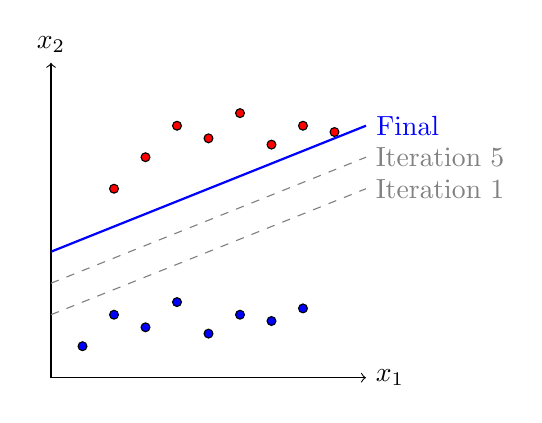
\begin{tikzpicture}[scale=0.8]
    % Coordinate axes
    \draw[->] (0,0) -- (5,0) node[right] {$x_1$};
    \draw[->] (0,0) -- (0,5) node[above] {$x_2$};
    
    % Data points (simplified representation)
    \foreach \x/\y in {0.5/0.5, 1/1, 1.5/0.8, 2/1.2, 2.5/0.7, 3/1, 3.5/0.9, 4/1.1}
        \draw[fill=blue] (\x,\y) circle (2pt);
    
    \foreach \x/\y in {1/3, 1.5/3.5, 2/4, 2.5/3.8, 3/4.2, 3.5/3.7, 4/4, 4.5/3.9}
        \draw[fill=red] (\x,\y) circle (2pt);
    
    % Decision boundaries at different iterations
    \draw[dashed, gray] (0,1) -- (5,3) node[right] {Iteration 1};
    \draw[dashed, gray] (0,1.5) -- (5,3.5) node[right] {Iteration 5};
    \draw[thick, blue] (0,2) -- (5,4) node[right] {Final};
\end{tikzpicture}
\caption{Illustration of Perceptron convergence on linearly separable data. The decision boundary evolves over iterations until it perfectly separates the classes.}
\end{figure}

\subsection{Perceptron Convergence Theorem}
A fundamental result for the Perceptron algorithm:

\fbox{
\begin{minipage}{\dimexpr\textwidth-2\fboxsep-2\fboxrule\relax}
\textbf{Perceptron Convergence Theorem}

If the training data is linearly separable, then:
\begin{itemize}
    \item The Perceptron algorithm will find a linear classifier with zero training error
    \item It will converge within a finite number of steps
\end{itemize}
\end{minipage}
}

However, the Perceptron algorithm has limitations:
\begin{itemize}
    \item It only works for linearly separable data
    \item It may find any linear separator that works, not necessarily the "best" one
    \item The solution depends on the order of processing the training examples
\end{itemize}

This raises an important question: Among all possible linear separators, which one should we choose?

\section{The Hard-Margin Support Vector Machine}

\subsection{The Margin Concept}
The margin of a linear classifier is the distance from the decision boundary to the nearest training point. A classifier with a large margin is likely to generalize better to unseen data.

\begin{figure}[h]
\centering
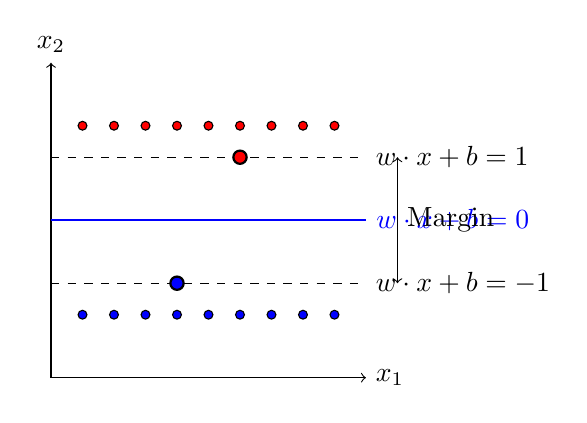
\begin{tikzpicture}[scale=0.8]
    % Coordinate axes
    \draw[->] (0,0) -- (5,0) node[right] {$x_1$};
    \draw[->] (0,0) -- (0,5) node[above] {$x_2$};
    
    % Decision boundary
    \draw[thick, blue] (0,2.5) -- (5,2.5) node[right] {$w \cdot x + b = 0$};
    
    % Margin boundaries
    \draw[dashed] (0,1.5) -- (5,1.5) node[right] {$w \cdot x + b = -1$};
    \draw[dashed] (0,3.5) -- (5,3.5) node[right] {$w \cdot x + b = 1$};
    
    % Margin
    \draw[<->] (5.5,1.5) -- (5.5,3.5) node[midway, right] {Margin};
    
    % Data points
    \foreach \x in {0.5,1,...,4.5}
        \draw[fill=blue] (\x,1) circle (2pt);
    
    \foreach \x in {0.5,1,...,4.5}
        \draw[fill=red] (\x,4) circle (2pt);
    
    % Support vectors
    \draw[fill=blue, thick] (2,1.5) circle (3pt);
    \draw[fill=red, thick] (3,3.5) circle (3pt);
\end{tikzpicture}
\caption{Illustration of the margin in a linearly separable dataset. The support vectors (highlighted) lie exactly on the margin boundaries.}
\end{figure}

\subsection{The Learning Problem}
Given training data $\{(x^{(i)}, y^{(i)}): i=1,\ldots,n\} \subset \mathbb{R}^d \times \{-1, +1\}$, we want to find $w \in \mathbb{R}^d$ and $b \in \mathbb{R}$ such that:
\begin{align}
y^{(i)}(w \cdot x^{(i)} + b) > 0 \quad \text{for all } i=1,\ldots,n
\end{align}

By scaling $w$ and $b$, we can equivalently require:
\begin{align}
y^{(i)}(w \cdot x^{(i)} + b) \geq 1 \quad \text{for all } i=1,\ldots,n
\end{align}

This formulation ensures that all points are not only correctly classified but also at least a certain distance from the decision boundary.

\subsection{Maximizing the Margin}
The margin $\gamma$ of a linear classifier is the distance from the decision boundary to the nearest training point. For a linear classifier with $\|w\| = 1$, this distance is given by $|w \cdot x + b|$.

With our constraint $y^{(i)}(w \cdot x^{(i)} + b) \geq 1$, the margin is $\gamma = 1/\|w\|$.

Therefore, maximizing the margin is equivalent to minimizing $\|w\|$, or equivalently, minimizing $\|w\|^2$ (which is differentiable everywhere).

\subsection{The Optimization Problem}
The hard-margin SVM optimization problem is:

\fbox{
\begin{minipage}{\dimexpr\textwidth-2\fboxsep-2\fboxrule\relax}
\textbf{Hard-Margin SVM Optimization Problem}

\begin{align}
\min_{w \in \mathbb{R}^d, b \in \mathbb{R}} & \|w\|^2 \\
\text{subject to: } & y^{(i)}(w \cdot x^{(i)} + b) \geq 1 \quad \text{for all } i = 1, 2, \ldots, n
\end{align}
\end{minipage}
}

This is a convex quadratic optimization problem with linear constraints, which means:
\begin{itemize}
    \item It has a unique global minimum
    \item It can be solved efficiently using standard optimization techniques
    \item Duality theory provides insights into the structure of the solution
\end{itemize}

\subsection{Support Vectors}
The solution to the SVM optimization problem has an interesting property: most training points have no influence on the decision boundary. The only points that matter are those that lie exactly on the margin, i.e., points for which $y^{(i)}(w \cdot x^{(i)} + b) = 1$. These points are called support vectors.

The optimal weight vector can be expressed as a linear combination of the support vectors:
\begin{align}
w = \sum_{i=1}^{n} \alpha_i y^{(i)} x^{(i)}
\end{align}
where $\alpha_i \geq 0$ are Lagrange multipliers that are non-zero only for support vectors.

\begin{figure}[h]
\centering
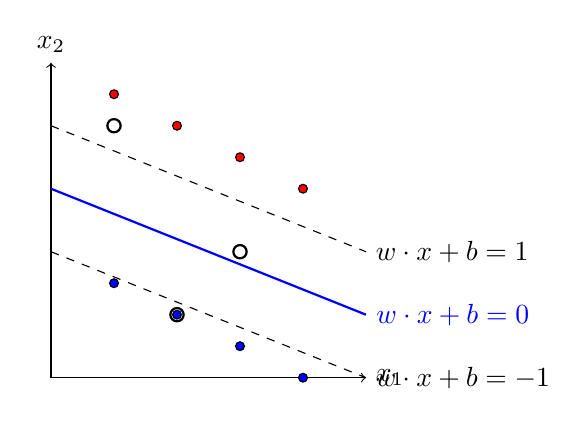
\begin{tikzpicture}[scale=0.8]
    % Coordinate axes
    \draw[->] (0,0) -- (5,0) node[right] {$x_1$};
    \draw[->] (0,0) -- (0,5) node[above] {$x_2$};
    
    % Decision boundary
    \draw[thick, blue] (0,3) -- (5,1) node[right] {$w \cdot x + b = 0$};
    
    % Margin boundaries
    \draw[dashed] (0,4) -- (5,2) node[right] {$w \cdot x + b = 1$};
    \draw[dashed] (0,2) -- (5,0) node[right] {$w \cdot x + b = -1$};
    
    % Data points
    \foreach \x/\y in {1/4.5, 2/4, 3/3.5, 4/3}
        \draw[fill=red] (\x,\y) circle (2pt);
    
    \foreach \x/\y in {1/1.5, 2/1, 3/0.5, 4/0}
        \draw[fill=blue] (\x,\y) circle (2pt);
    
    % Support vectors
    \draw[thick] (1,4) circle (3pt);
    \draw[thick] (3,2) circle (3pt);
    \draw[thick] (2,1) circle (3pt);
\end{tikzpicture}
\caption{Support vectors are the points that lie exactly on the margin boundaries. The decision boundary is determined entirely by these points.}
\end{figure}

\section{Example: Iris Dataset}

\subsection{Dataset Description}
The Iris dataset is a classic dataset in machine learning, collected by the botanist Edgar Anderson and made famous by the statistician Ronald Fisher. It contains measurements of 150 iris flowers from three different species:

\begin{itemize}
    \item Iris setosa
    \item Iris versicolor
    \item Iris virginica
\end{itemize}

For each flower, four measurements were taken:
\begin{itemize}
    \item Sepal length
    \item Sepal width
    \item Petal length
    \item Petal width
\end{itemize}

\subsection{Binary Classification Example}
For simplicity, we can consider a binary classification problem using only two of the species (setosa and versicolor) and two of the features (sepal width and petal width).

\begin{figure}[h]
\centering
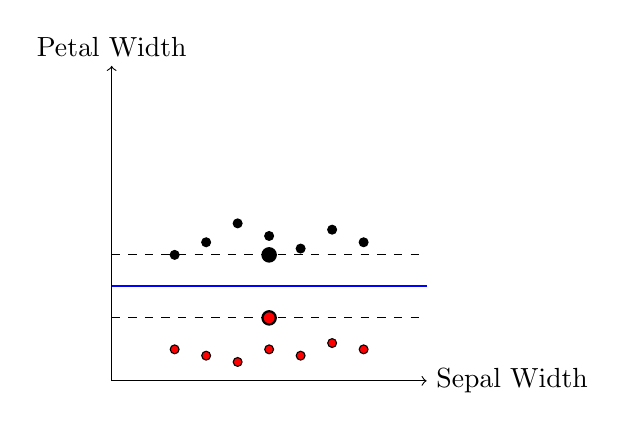
\begin{tikzpicture}[scale=0.8]
    % Coordinate axes
    \draw[->] (0,0) -- (5,0) node[right] {Sepal Width};
    \draw[->] (0,0) -- (0,5) node[above] {Petal Width};
    
    % Setosa (red circles)
    \foreach \x/\y in {1/0.5, 1.5/0.4, 2/0.3, 2.5/0.5, 3/0.4, 3.5/0.6, 4/0.5}
        \draw[fill=red] (\x,\y) circle (2pt);
    
    % Versicolor (black triangles)
    \foreach \x/\y in {1/2, 1.5/2.2, 2/2.5, 2.5/2.3, 3/2.1, 3.5/2.4, 4/2.2}
        \draw[fill=black] (\x,\y) circle (2pt);
    
    % Decision boundary
    \draw[thick, blue] (0,1.5) -- (5,1.5);
    
    % Margin boundaries
    \draw[dashed] (0,1) -- (5,1);
    \draw[dashed] (0,2) -- (5,2);
    
    % Support vectors
    \draw[fill=red, thick] (2.5,1) circle (3pt);
    \draw[fill=black, thick] (2.5,2) circle (3pt);
\end{tikzpicture}
\caption{SVM classification of Iris setosa (red circles) and Iris versicolor (black triangles) using sepal width and petal width features.}
\end{figure}

In this example, the data is linearly separable, and the SVM finds the maximum-margin linear classifier. The support vectors are the points that lie exactly on the margin boundaries.

\section{The Soft-Margin SVM}

\subsection{Handling Non-linearly Separable Data}
The hard-margin SVM assumes that the data is linearly separable. However, in real-world scenarios, data is often not perfectly separable due to noise or outliers. To handle such cases, we can use a soft-margin SVM, which allows for some misclassifications.

\subsection{Slack Variables}
We introduce slack variables $\xi_i \geq 0$ for each training point, which measure the degree of misclassification:

\begin{align}
y^{(i)}(w \cdot x^{(i)} + b) \geq 1 - \xi_i \quad \text{for all } i = 1, 2, \ldots, n
\end{align}

The interpretation of $\xi_i$ is:
\begin{itemize}
    \item $\xi_i = 0$: The point is correctly classified and on or beyond the margin
    \item $0 < \xi_i \leq 1$: The point is correctly classified but within the margin
    \item $\xi_i > 1$: The point is misclassified
\end{itemize}

\subsection{The Optimization Problem}
The soft-margin SVM optimization problem is:

\fbox{
\begin{minipage}{\dimexpr\textwidth-2\fboxsep-2\fboxrule\relax}
\textbf{Soft-Margin SVM Optimization Problem}

\begin{align}
\min_{w \in \mathbb{R}^d, b \in \mathbb{R}, \xi \in \mathbb{R}^n} & \|w\|^2 + C \sum_{i=1}^{n} \xi_i \\
\text{subject to: } & y^{(i)}(w \cdot x^{(i)} + b) \geq 1 - \xi_i \quad \text{for all } i = 1, 2, \ldots, n \\
& \xi_i \geq 0 \quad \text{for all } i = 1, 2, \ldots, n
\end{align}
\end{minipage}
}

The parameter $C > 0$ controls the trade-off between maximizing the margin and minimizing the classification error. A larger $C$ places more emphasis on correctly classifying all training points, while a smaller $C$ places more emphasis on maximizing the margin.

\begin{figure}[h]
\centering
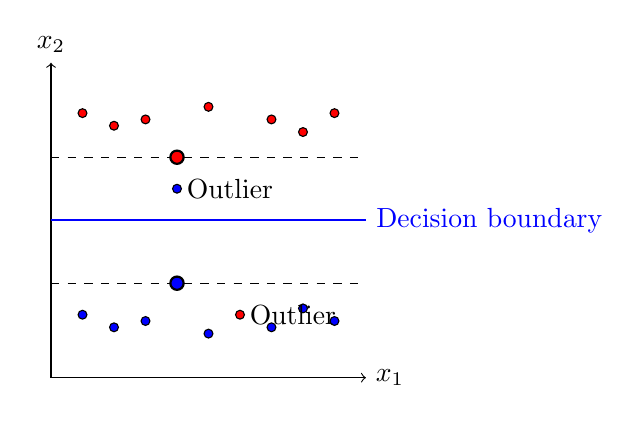
\begin{tikzpicture}[scale=0.8]
    % Coordinate axes
    \draw[->] (0,0) -- (5,0) node[right] {$x_1$};
    \draw[->] (0,0) -- (0,5) node[above] {$x_2$};
    
    % Decision boundary
    \draw[thick, blue] (0,2.5) -- (5,2.5) node[right] {Decision boundary};
    
    % Margin boundaries
    \draw[dashed] (0,1.5) -- (5,1.5);
    \draw[dashed] (0,3.5) -- (5,3.5);
    
    % Data points
    \foreach \x/\y in {0.5/1, 1/0.8, 1.5/0.9, 2.5/0.7, 3.5/0.8, 4/1.1, 4.5/0.9}
        \draw[fill=blue] (\x,\y) circle (2pt);
    
    \foreach \x/\y in {0.5/4.2, 1/4, 1.5/4.1, 2.5/4.3, 3.5/4.1, 4/3.9, 4.5/4.2}
        \draw[fill=red] (\x,\y) circle (2pt);
    
    % Outliers
    \draw[fill=blue] (2,3) circle (2pt) node[right] {Outlier};
    \draw[fill=red] (3,1) circle (2pt) node[right] {Outlier};
    
    % Support vectors
    \draw[fill=blue, thick] (2,1.5) circle (3pt);
    \draw[fill=red, thick] (2,3.5) circle (3pt);
\end{tikzpicture}
\caption{Soft-margin SVM allows for some misclassifications to handle outliers or non-linearly separable data.}
\end{figure}

\section{Parameter Selection for SVMs}

\subsection{The Role of Parameter $C$}
The parameter $C$ in the soft-margin SVM formulation controls the trade-off between maximizing the margin and minimizing the classification error:

\begin{itemize}
    \item Small $C$: Places more emphasis on maximizing the margin, even if it means allowing more training errors
    \item Large $C$: Places more emphasis on minimizing training errors, potentially at the cost of a smaller margin
\end{itemize}

\begin{figure}[h]
\centering
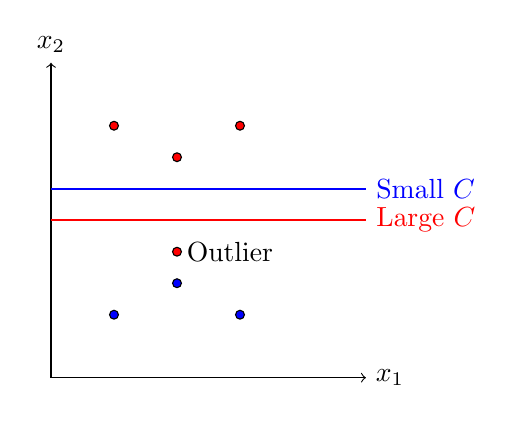
\begin{tikzpicture}[scale=0.8]
    % Coordinate axes
    \draw[->] (0,0) -- (5,0) node[right] {$x_1$};
    \draw[->] (0,0) -- (0,5) node[above] {$x_2$};
    
    % Data points
    \draw[fill=red] (1,4) circle (2pt);
    \draw[fill=red] (2,3.5) circle (2pt);
    \draw[fill=red] (3,4) circle (2pt);
    \draw[fill=blue] (1,1) circle (2pt);
    \draw[fill=blue] (2,1.5) circle (2pt);
    \draw[fill=blue] (3,1) circle (2pt);
    
    % Outlier
    \draw[fill=red] (2,2) circle (2pt) node[right] {Outlier};
    
    % Decision boundaries
    \draw[thick, blue] (0,3) -- (5,3) node[right] {Small $C$};
    \draw[thick, red] (0,2.5) -- (5,2.5) node[right] {Large $C$};
\end{tikzpicture}
\caption{Effect of parameter $C$ on the decision boundary. A small $C$ (blue line) allows the outlier to be misclassified to maintain a larger margin. A large $C$ (red line) adjusts the boundary to correctly classify the outlier, resulting in a smaller margin.}
\end{figure}

\subsection{Practical Implications}
The choice of $C$ has significant practical implications:

\begin{itemize}
    \item \textbf{Overfitting vs. Underfitting}: Large $C$ values can lead to overfitting, while small $C$ values might result in underfitting
    \item \textbf{Number of Support Vectors}: Larger $C$ values typically result in fewer support vectors
    \item \textbf{Generalization Performance}: The optimal $C$ value balances training accuracy and generalization to unseen data
\end{itemize}

\section{Sentiment Analysis Example}

\subsection{Dataset Description}
To illustrate the importance of parameter selection, we'll examine a sentiment analysis dataset:

\begin{itemize}
    \item \textbf{Source}: Reviews from Amazon, Yelp, and IMDB
    \item \textbf{Labels}: Binary classification (positive or negative sentiment)
    \item \textbf{Representation}: Bag-of-words with a vocabulary of 4500 words
    \item \textbf{Size}: 2500 training sentences, 500 test sentences
\end{itemize}

\subsection{Example Sentences}
The dataset contains sentences like:

\begin{itemize}
    \item "Needless to say, I wasted my money." (Negative)
    \item "He was very impressed when going from the original battery to the extended battery." (Positive)
    \item "I have to jiggle the plug to get it to line up right to get decent volume." (Negative)
    \item "Will order from them again!" (Positive)
\end{itemize}

\subsection{Feature Representation}
The bag-of-words representation transforms each sentence into a high-dimensional vector:

\begin{itemize}
    \item Each dimension corresponds to a word in the vocabulary
    \item The value in each dimension represents the presence or frequency of the word in the sentence
    \item This creates a sparse vector representation (most entries are zero)
\end{itemize}

\begin{figure}[h]
\centering
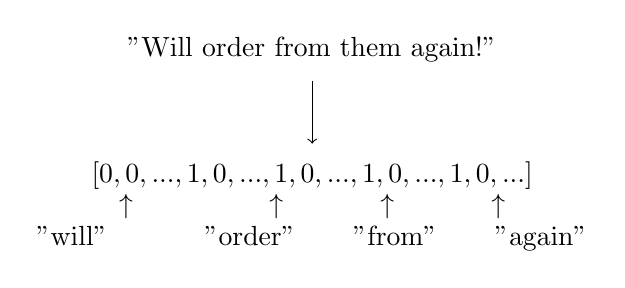
\begin{tikzpicture}[scale=0.8]
    % Sentence
    \node[align=left] at (0,4) {"Will order from them again!"};
    
    % Arrow
    \draw[->] (0,3.5) -- (0,2.5);
    
    % Vector representation
    \node[align=left] at (0,2) {$[0, 0, ..., 1, 0, ..., 1, 0, ..., 1, 0, ..., 1, 0, ...]$};
    \node[align=left] at (0,1.5) {$\uparrow$ \hspace{1.5cm} $\uparrow$ \hspace{1cm} $\uparrow$ \hspace{1cm} $\uparrow$};
    \node[align=left] at (0,1) {"will" \hspace{1cm} "order" \hspace{0.5cm} "from" \hspace{0.5cm} "again"};
\end{tikzpicture}
\caption{Bag-of-words representation of a sentence. Each word in the vocabulary corresponds to a dimension in the feature vector.}
\end{figure}

\section{Experimental Results with Different $C$ Values}

\subsection{Performance Metrics}
For each value of $C$, we measure three key metrics:

\begin{itemize}
    \item \textbf{Training error}: Percentage of misclassified training examples
    \item \textbf{Test error}: Percentage of misclassified test examples
    \item \textbf{Number of support vectors}: Points that influence the decision boundary
\end{itemize}

\subsection{Results Table}
\begin{table}[h]
\centering
\begin{tabular}{|c|c|c|c|}
\hline
\textbf{C} & \textbf{Training Error (\%)} & \textbf{Test Error (\%)} & \textbf{\# Support Vectors} \\
\hline
0.01 & 23.72 & 28.4 & 2294 \\
0.1 & 7.88 & 18.4 & 1766 \\
1 & 1.12 & 16.8 & 1306 \\
10 & 0.16 & 19.4 & 1105 \\
100 & 0.08 & 19.4 & 1035 \\
1000 & 0.08 & 19.4 & 950 \\
\hline
\end{tabular}
\caption{Performance metrics for different values of parameter $C$ on the sentiment analysis dataset}
\end{table}

\subsection{Analysis of Results}
Several important trends can be observed from the experimental results:

\begin{enumerate}
    \item \textbf{Training Error}: Decreases monotonically as $C$ increases
    \begin{itemize}
        \item At $C = 0.01$: High training error (23.72\%)
        \item At $C = 1000$: Near-zero training error (0.08\%)
    \end{itemize}
    
    \item \textbf{Test Error}: Initially decreases as $C$ increases, then increases
    \begin{itemize}
        \item At $C = 0.01$: High test error (28.4\%)
        \item At $C = 1$: Lowest test error (16.8\%)
        \item At $C \geq 10$: Test error increases to 19.4\%
    \end{itemize}
    
    \item \textbf{Number of Support Vectors}: Decreases as $C$ increases
    \begin{itemize}
        \item At $C = 0.01$: Many support vectors (2294)
        \item At $C = 1000$: Fewer support vectors (950)
    \end{itemize}
\end{enumerate}

\begin{figure}[h]
\centering
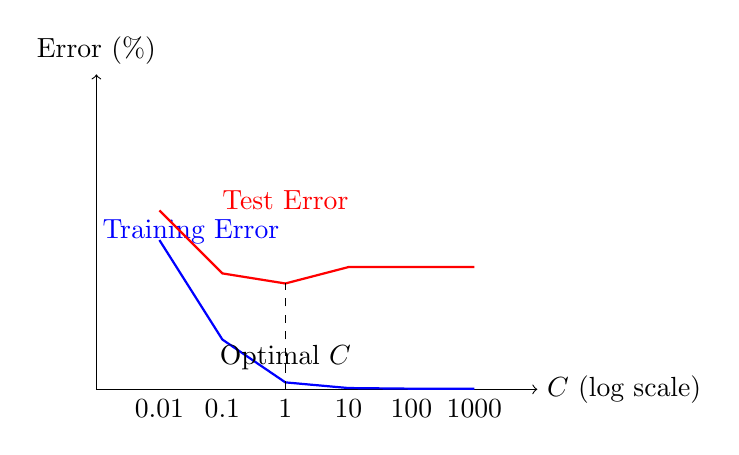
\begin{tikzpicture}[scale=0.8]
    % Coordinate axes
    \draw[->] (0,0) -- (7,0) node[right] {$C$ (log scale)};
    \draw[->] (0,0) -- (0,5) node[above] {Error (\%)};
    
    % X-axis labels
    \node at (1,-0.3) {0.01};
    \node at (2,-0.3) {0.1};
    \node at (3,-0.3) {1};
    \node at (4,-0.3) {10};
    \node at (5,-0.3) {100};
    \node at (6,-0.3) {1000};
    
    % Training error
    \draw[thick, blue] (1,2.37) -- (2,0.79) -- (3,0.11) -- (4,0.02) -- (5,0.01) -- (6,0.01);
    \node[blue] at (1.5,2.5) {Training Error};
    
    % Test error
    \draw[thick, red] (1,2.84) -- (2,1.84) -- (3,1.68) -- (4,1.94) -- (5,1.94) -- (6,1.94);
    \node[red] at (3,3) {Test Error};
    
    % Optimal C
    \draw[dashed] (3,0) -- (3,1.68);
    \node at (3,0.5) {Optimal $C$};
\end{tikzpicture}
\caption{Training and test error as a function of parameter $C$ (log scale). The optimal $C$ value minimizes the test error.}
\end{figure}

\section{Cross-Validation for Parameter Tuning}

\subsection{The Cross-Validation Procedure}
To find the optimal value of $C$, we can use cross-validation:

\begin{enumerate}
    \item Divide the training data into $k$ equal folds (e.g., $k = 5$)
    \item For each value of $C$:
    \begin{enumerate}
        \item For each fold $i$ (from 1 to $k$):
        \begin{enumerate}
            \item Train an SVM on all folds except fold $i$
            \item Evaluate the model on fold $i$
        \end{enumerate}
        \item Calculate the average error across all $k$ folds
    \end{enumerate}
    \item Select the $C$ value with the lowest average error
\end{enumerate}

\begin{figure}[h]
\centering
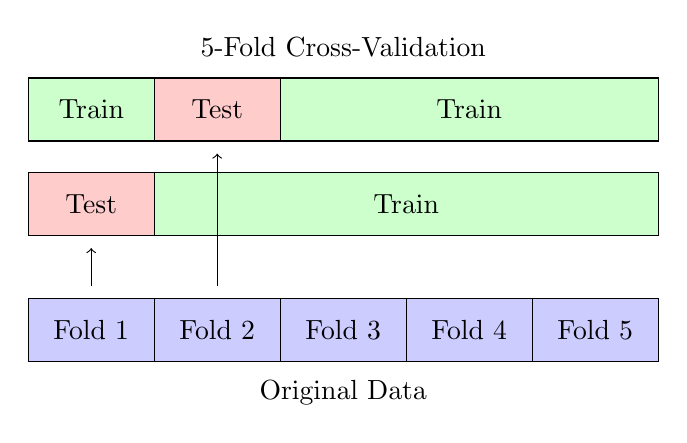
\begin{tikzpicture}[scale=0.8]
    % Data folds
    \draw[fill=blue!20] (0,0) rectangle (2,1) node[pos=0.5] {Fold 1};
    \draw[fill=blue!20] (2,0) rectangle (4,1) node[pos=0.5] {Fold 2};
    \draw[fill=blue!20] (4,0) rectangle (6,1) node[pos=0.5] {Fold 3};
    \draw[fill=blue!20] (6,0) rectangle (8,1) node[pos=0.5] {Fold 4};
    \draw[fill=blue!20] (8,0) rectangle (10,1) node[pos=0.5] {Fold 5};
    
    % Iteration 1
    \draw[fill=red!20] (0,2) rectangle (2,3) node[pos=0.5] {Test};
    \draw[fill=green!20] (2,2) rectangle (10,3) node[pos=0.5] {Train};
    
    % Iteration 2
    \draw[fill=green!20] (0,3.5) rectangle (2,4.5) node[pos=0.5] {Train};
    \draw[fill=red!20] (2,3.5) rectangle (4,4.5) node[pos=0.5] {Test};
    \draw[fill=green!20] (4,3.5) rectangle (10,4.5) node[pos=0.5] {Train};
    
    % Arrows
    \draw[->] (1,1.2) -- (1,1.8);
    \draw[->] (3,1.2) -- (3,3.3);
    
    % Labels
    \node at (5,-0.5) {Original Data};
    \node at (5,5) {5-Fold Cross-Validation};
\end{tikzpicture}
\caption{Illustration of 5-fold cross-validation. The data is divided into 5 folds, and each fold serves as the test set once while the remaining folds form the training set.}
\end{figure}

\subsection{Cross-Validation Results}
For the sentiment analysis dataset, 5-fold cross-validation was performed to select the optimal $C$ value:

\begin{itemize}
    \item The optimal value was found to be $C = 0.32$
    \item With this value, the test error was 15.6\%
\end{itemize}

This is better than any of the individual $C$ values tested in the previous experiment, highlighting the importance of proper parameter tuning.

\section{Interpreting the Trade-offs}

\subsection{Bias-Variance Trade-off}
The results illustrate the classic bias-variance trade-off in machine learning:

\begin{itemize}
    \item \textbf{Small $C$ values} (e.g., $C = 0.01$):
    \begin{itemize}
        \item High bias (underfitting)
        \item Simple model with large margin
        \item High training and test error
    \end{itemize}
    
    \item \textbf{Large $C$ values} (e.g., $C = 1000$):
    \begin{itemize}
        \item High variance (overfitting)
        \item Complex model with small margin
        \item Low training error but higher test error
    \end{itemize}
    
    \item \textbf{Optimal $C$ value} (e.g., $C = 0.32$ from cross-validation):
    \begin{itemize}
        \item Balances bias and variance
        \item Moderate margin size
        \item Best generalization performance
    \end{itemize}
\end{itemize}

\subsection{Margin vs. Classification Accuracy}
The parameter $C$ controls the trade-off between margin size and classification accuracy:

\begin{itemize}
    \item \textbf{Small $C$}: Prioritizes larger margins at the expense of training accuracy
    \item \textbf{Large $C$}: Prioritizes training accuracy at the expense of margin size
\end{itemize}

\subsection{Model Complexity}
The number of support vectors is an indicator of model complexity:

\begin{itemize}
    \item More support vectors generally mean a more complex model
    \item As $C$ increases, the number of support vectors decreases
    \item However, too few support vectors might indicate overfitting to the training data
\end{itemize}

\section{Practical Considerations}

\subsection{Feature Scaling}
SVMs are sensitive to the scale of the features. It's generally recommended to scale the features before training an SVM:

\begin{itemize}
    \item \textbf{Standardization}: $x' = \frac{x - \mu}{\sigma}$
    \item \textbf{Min-max scaling}: $x' = \frac{x - \min(x)}{\max(x) - \min(x)}$
\end{itemize}

\subsection{Handling Large Datasets}
Standard SVM implementations have time complexity $O(n^2)$ to $O(n^3)$, where $n$ is the number of training examples. This can be prohibitive for large datasets. Several approaches exist for scaling SVMs to large datasets:

\begin{itemize}
    \item \textbf{Chunking}: Solve the optimization problem in smaller chunks
    \item \textbf{Sequential Minimal Optimization (SMO)}: Optimize two Lagrange multipliers at a time
    \item \textbf{Stochastic gradient descent}: Approximate the SVM solution using SGD
    \item \textbf{Linear SVMs}: For linear kernels, specialized algorithms like LIBLINEAR can scale to millions of examples
\end{itemize}

\subsection{Kernel Selection}
While linear SVMs are effective for many high-dimensional problems (like text classification), non-linear kernels can be useful for other types of data:

\begin{itemize}
    \item \textbf{Linear kernel}: $K(x, z) = x \cdot z$
    \item \textbf{Polynomial kernel}: $K(x, z) = (x \cdot z + c)^d$
    \item \textbf{Radial Basis Function (RBF) kernel}: $K(x, z) = \exp(-\gamma \|x - z\|^2)$
    \item \textbf{Sigmoid kernel}: $K(x, z) = \tanh(\alpha x \cdot z + c)$
\end{itemize}

\subsection{Multi-class Classification}
SVMs are inherently binary classifiers, but they can be extended to multi-class problems using several strategies:

\begin{itemize}
    \item \textbf{One-vs-Rest}: Train $k$ binary SVMs, each separating one class from the rest
    \item \textbf{One-vs-One}: Train $\binom{k}{2}$ binary SVMs, one for each pair of classes
    \item \textbf{Direct Multi-class Formulation}: Extend the SVM optimization problem to directly handle multiple classes
\end{itemize}

\section{Summary and Key Takeaways}

\subsection{Linear Classification Approaches}
We've explored several approaches to linear classification:

\begin{itemize}
    \item \textbf{Perceptron}: A simple, iterative algorithm that finds any linear separator for linearly separable data
    \item \textbf{Hard-margin SVM}: Finds the maximum-margin linear separator for linearly separable data
    \item \textbf{Soft-margin SVM}: Extends the hard-margin SVM to handle non-linearly separable data by allowing some misclassifications
\end{itemize}

\subsection{The Importance of Parameter Tuning}
The soft-margin SVM parameter $C$ controls the trade-off between margin size and classification accuracy:

\begin{itemize}
    \item Small $C$ values prioritize larger margins, potentially allowing more training errors
    \item Large $C$ values prioritize minimizing training errors, potentially at the cost of smaller margins
    \item The optimal $C$ value balances these trade-offs to achieve the best generalization performance
    \item Cross-validation is an effective method for selecting the optimal $C$ value
\end{itemize}

\subsection{Practical Guidelines}
Based on our exploration, here are some practical guidelines for using linear classifiers:

\begin{itemize}
    \item \textbf{Start with a linear SVM}: For many problems, especially high-dimensional ones like text classification, a linear SVM is a good baseline
    \item \textbf{Use cross-validation for parameter tuning}: Test a range of $C$ values (e.g., $10^{-2}$ to $10^3$) and select the one with the best validation performance
    \item \textbf{Monitor both training and test performance}: This helps identify underfitting or overfitting
    \item \textbf{Consider the number of support vectors}: Too many might indicate underfitting, while too few might indicate overfitting
    \item \textbf{Scale features appropriately}: SVMs are sensitive to the scale of the features
    \item \textbf{For non-linear problems}: Consider using kernel SVMs or other non-linear classifiers
\end{itemize}

\subsection{Future Directions}
Linear classification continues to be an active area of research and development:

\begin{itemize}
    \item \textbf{Scalable algorithms}: Developing more efficient algorithms for large-scale linear classification
    \item \textbf{Online learning}: Adapting linear classifiers for streaming data
    \item \textbf{Deep learning}: Combining linear classifiers with deep neural networks
    \item \textbf{Interpretability}: Enhancing the interpretability of linear classifiers for complex domains
\end{itemize}

\end{document}